%!TEX root = ../../super_main.tex

\chapter{User Interfaces}
\label{cha:user_interfaces}

In order to enable participants to contribute to campaigns they need a way to interact with the system, and customers need to be able to create the campaigns that the participants should contribute to. Furthermore, customers need a way to retrieve the collected information for their campaigns. All of the interfaces of uMiner and a description of how to interact with them is covered in this chapter. When designing these various screens we have utilized mockups as a creative tool to prototype different layouts prior to implementing them. The mockups for the participants interaction is shown along side the implementation in \secref{sec:participant_interaction}. The mockups for the customer interaction can be, because of their size, found in \appref{app:web_mockup}.

%!TEX root = ../../super_main.tex

\section{Participant Interaction}
\label{sec:participant_interaction}
Limited screen real estate characterizes user interfaces for mobile systems and is a general concern when designing user interfaces for these, compared to designing GUIs for desktop systems \parencite[cha. 21]{mobile_computing_constraints}. The limited screen real estate is generally solved by more navigation and by having more focus on a few visible elements at a time. We have therefore split our graphical user interface into a few logical screens and implemented navigation between them in order to improve the interaction. Having all functionality on one screen tends to be less portable to many different screen sizes and cause overlapping hit areas for buttons and other interactive elements.
\\\\
During the construction of the participant interface we have followed the Google Material Design\footnote{https://www.google.com/design/spec/material-design/} manual, which is a design manual provided by Google for the Android platform. This design manual helps designing an interface using good design practices on the Android platform. By adhering to this design manual, we hope to achieve a user friendly interface for participants that fits as many different users as possible. This will guide us in improving different aspects of our application, such as utilization of screen estate and usability in general without having to design an interface from the ground up.

\subsection{Opening the Application}
\label{sub:opening_the_application}
When a participant opens the mobile application, the participant is presented with an initial screen, as seen in \figref{fig:initial_screen}. The idea with this screen is to welcome the participant to the application. Currently, it does not supply the participant with any information, but one could imagine that this screen would, in a potential future release, provide the participant with usable information, such as progress in the current campaign, clarification of what concepts and principals the participant must know. This screen could possibly also contain some motivational factor, provided by the customers, e.g. a ``prize'' for participation.

% Initial screen
\begin{figure}[!htbp]
    \begin{subfigure}[!t]{.48\textwidth}
        \centering
        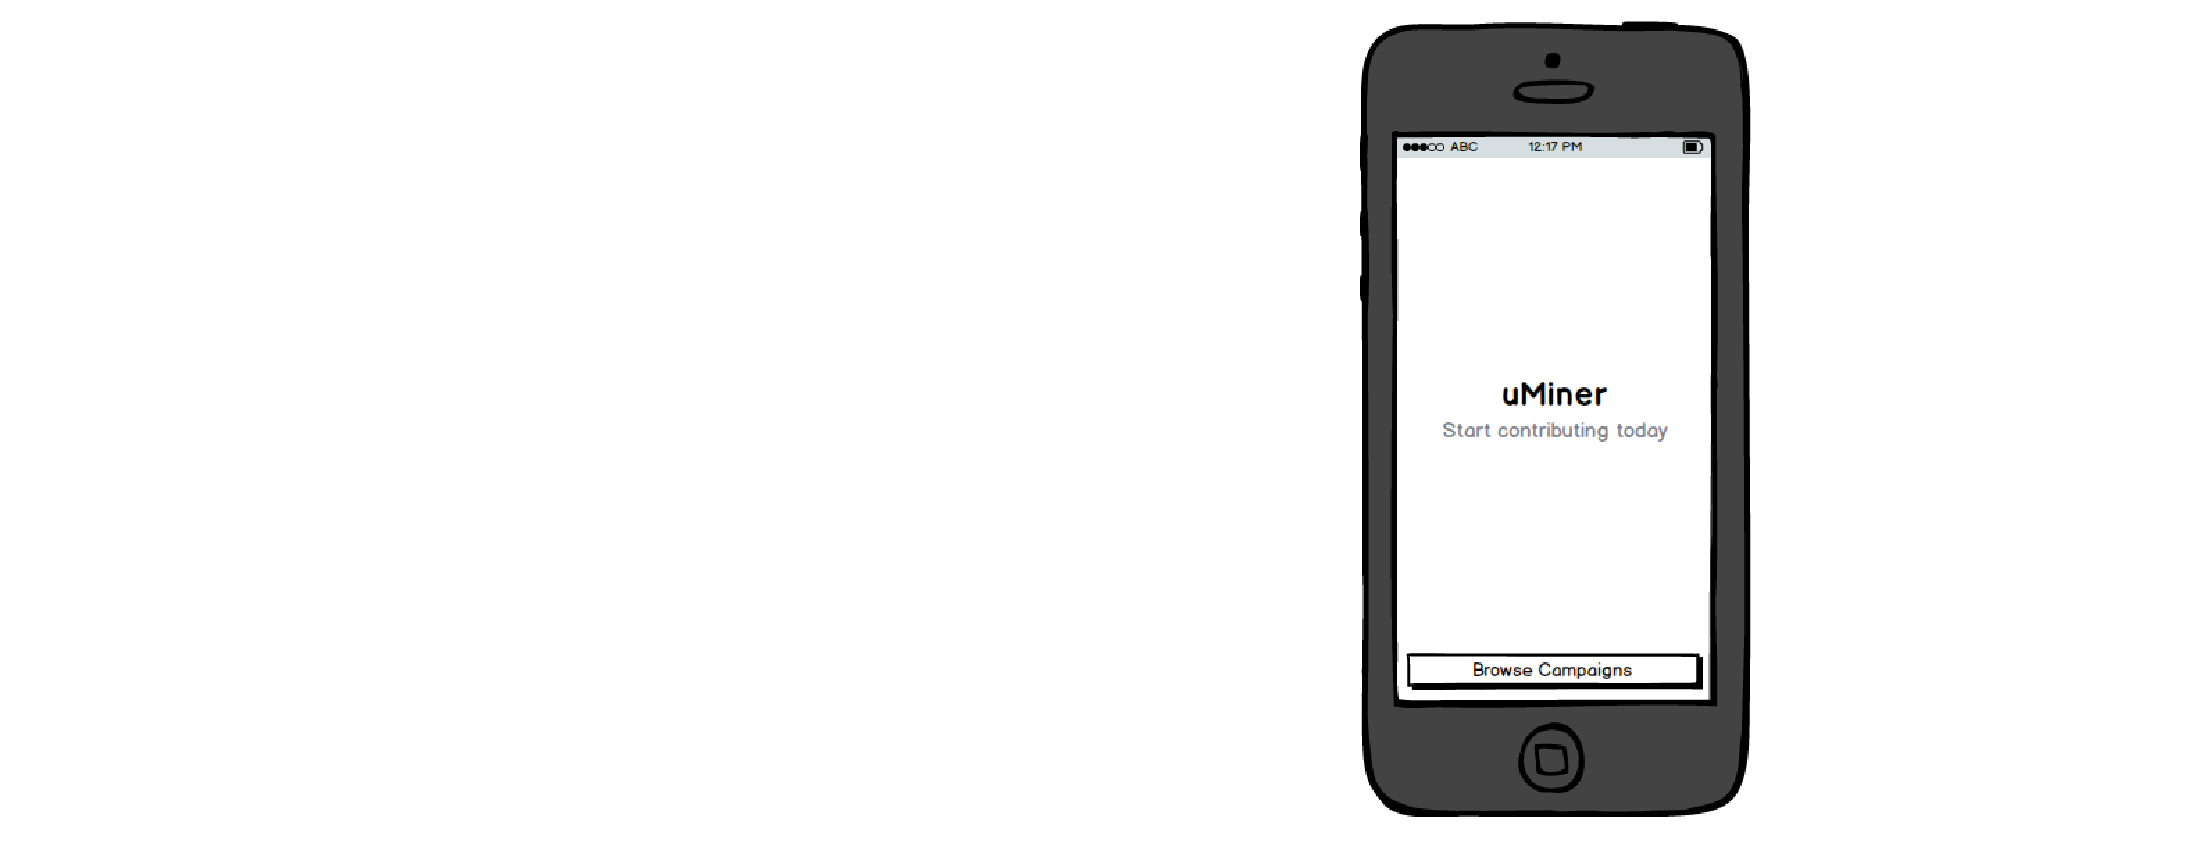
\includegraphics[width=.7\linewidth]{mockups/homepage}
        \caption{Mockup of the initial screen.}
        \label{fig:mockup_initial_screen}
    \end{subfigure}%
    \begin{subfigure}[!t]{.52\textwidth}
    \centering
        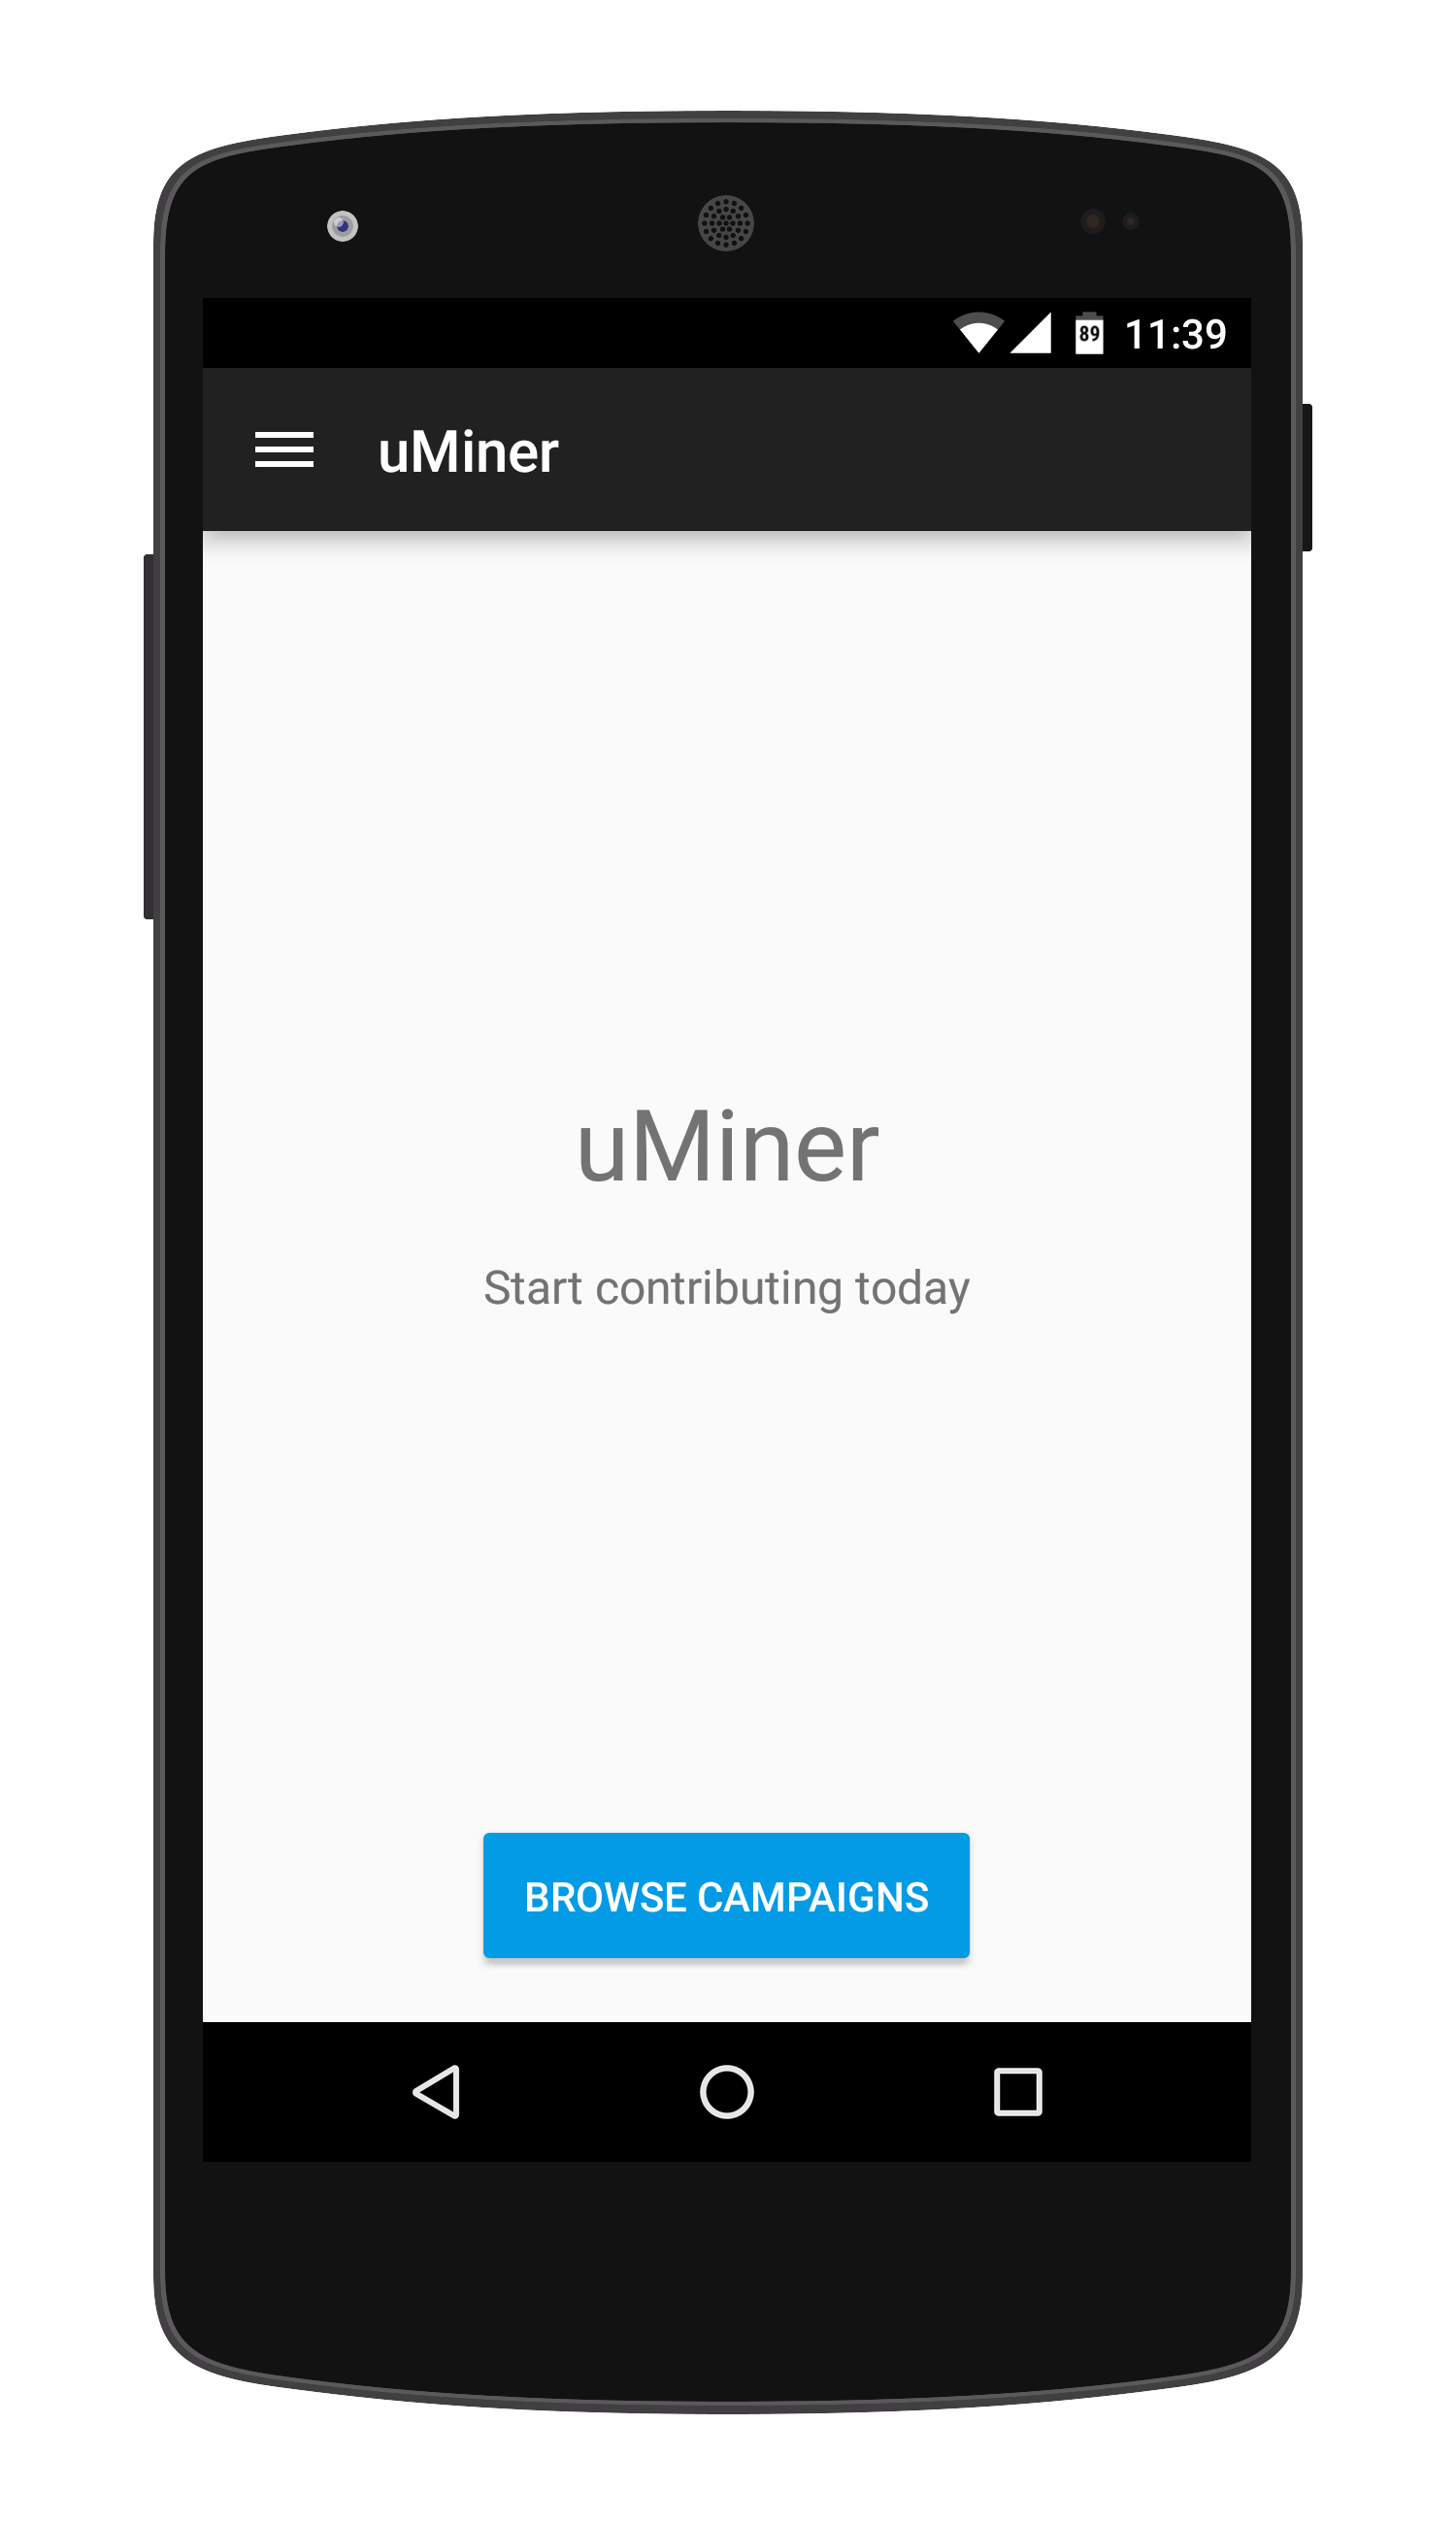
\includegraphics[width=.73\linewidth]{user_interfaces/client/client_uminer_home_with_phone}
        \caption{Implementation of the initial screen.}
        \label{fig:implementation_initial_screen}
    \end{subfigure}
    \caption{Mockup and implementation of the initial screen of the application.}
    \label{fig:initial_screen}
\end{figure}
\FloatBarrier

The participants must either use the drawer menu displayed in \figref{fig:navigation} or press the \emph{browse campaigns}-button in the initial screen to navigate to other parts of the application. The navigation menu contains three elements, namely ``Browse campaigns'', ``Join specific'', and ``Current campaign'', which each takes the participant to different parts of the application. This menu will at all times be available in the primary application by swiping from the left edge of the screen, or by pressing the hamburger icon ($\equiv$) next to the uMiner title in the top bar. 

\begin{description}
    \item[``Browse campaigns''] redirects the participant to a view containing brief information about all of the publicly available campaigns, as seen in \figref{fig:public_campaigns}.

    \item[``Join specific''] redirects the participant to a screen, as seen in \figref{fig:specific_campaign}, where it is possible to search for a specific campaign by providing a campaign identifier.

    \item[``Current campaign''] redirects the participant to a campaign specification screen, as seen in \figref{fig:leave_campaign_no_dialog}, displaying more information about the campaign that they are currently contributing to. If the participant have not yet joined a campaign, a message will briefly be displayed on the screen, informing the participant about this.
\end{description}

% Navigation
\begin{figure}[!htbp]
    \centering
    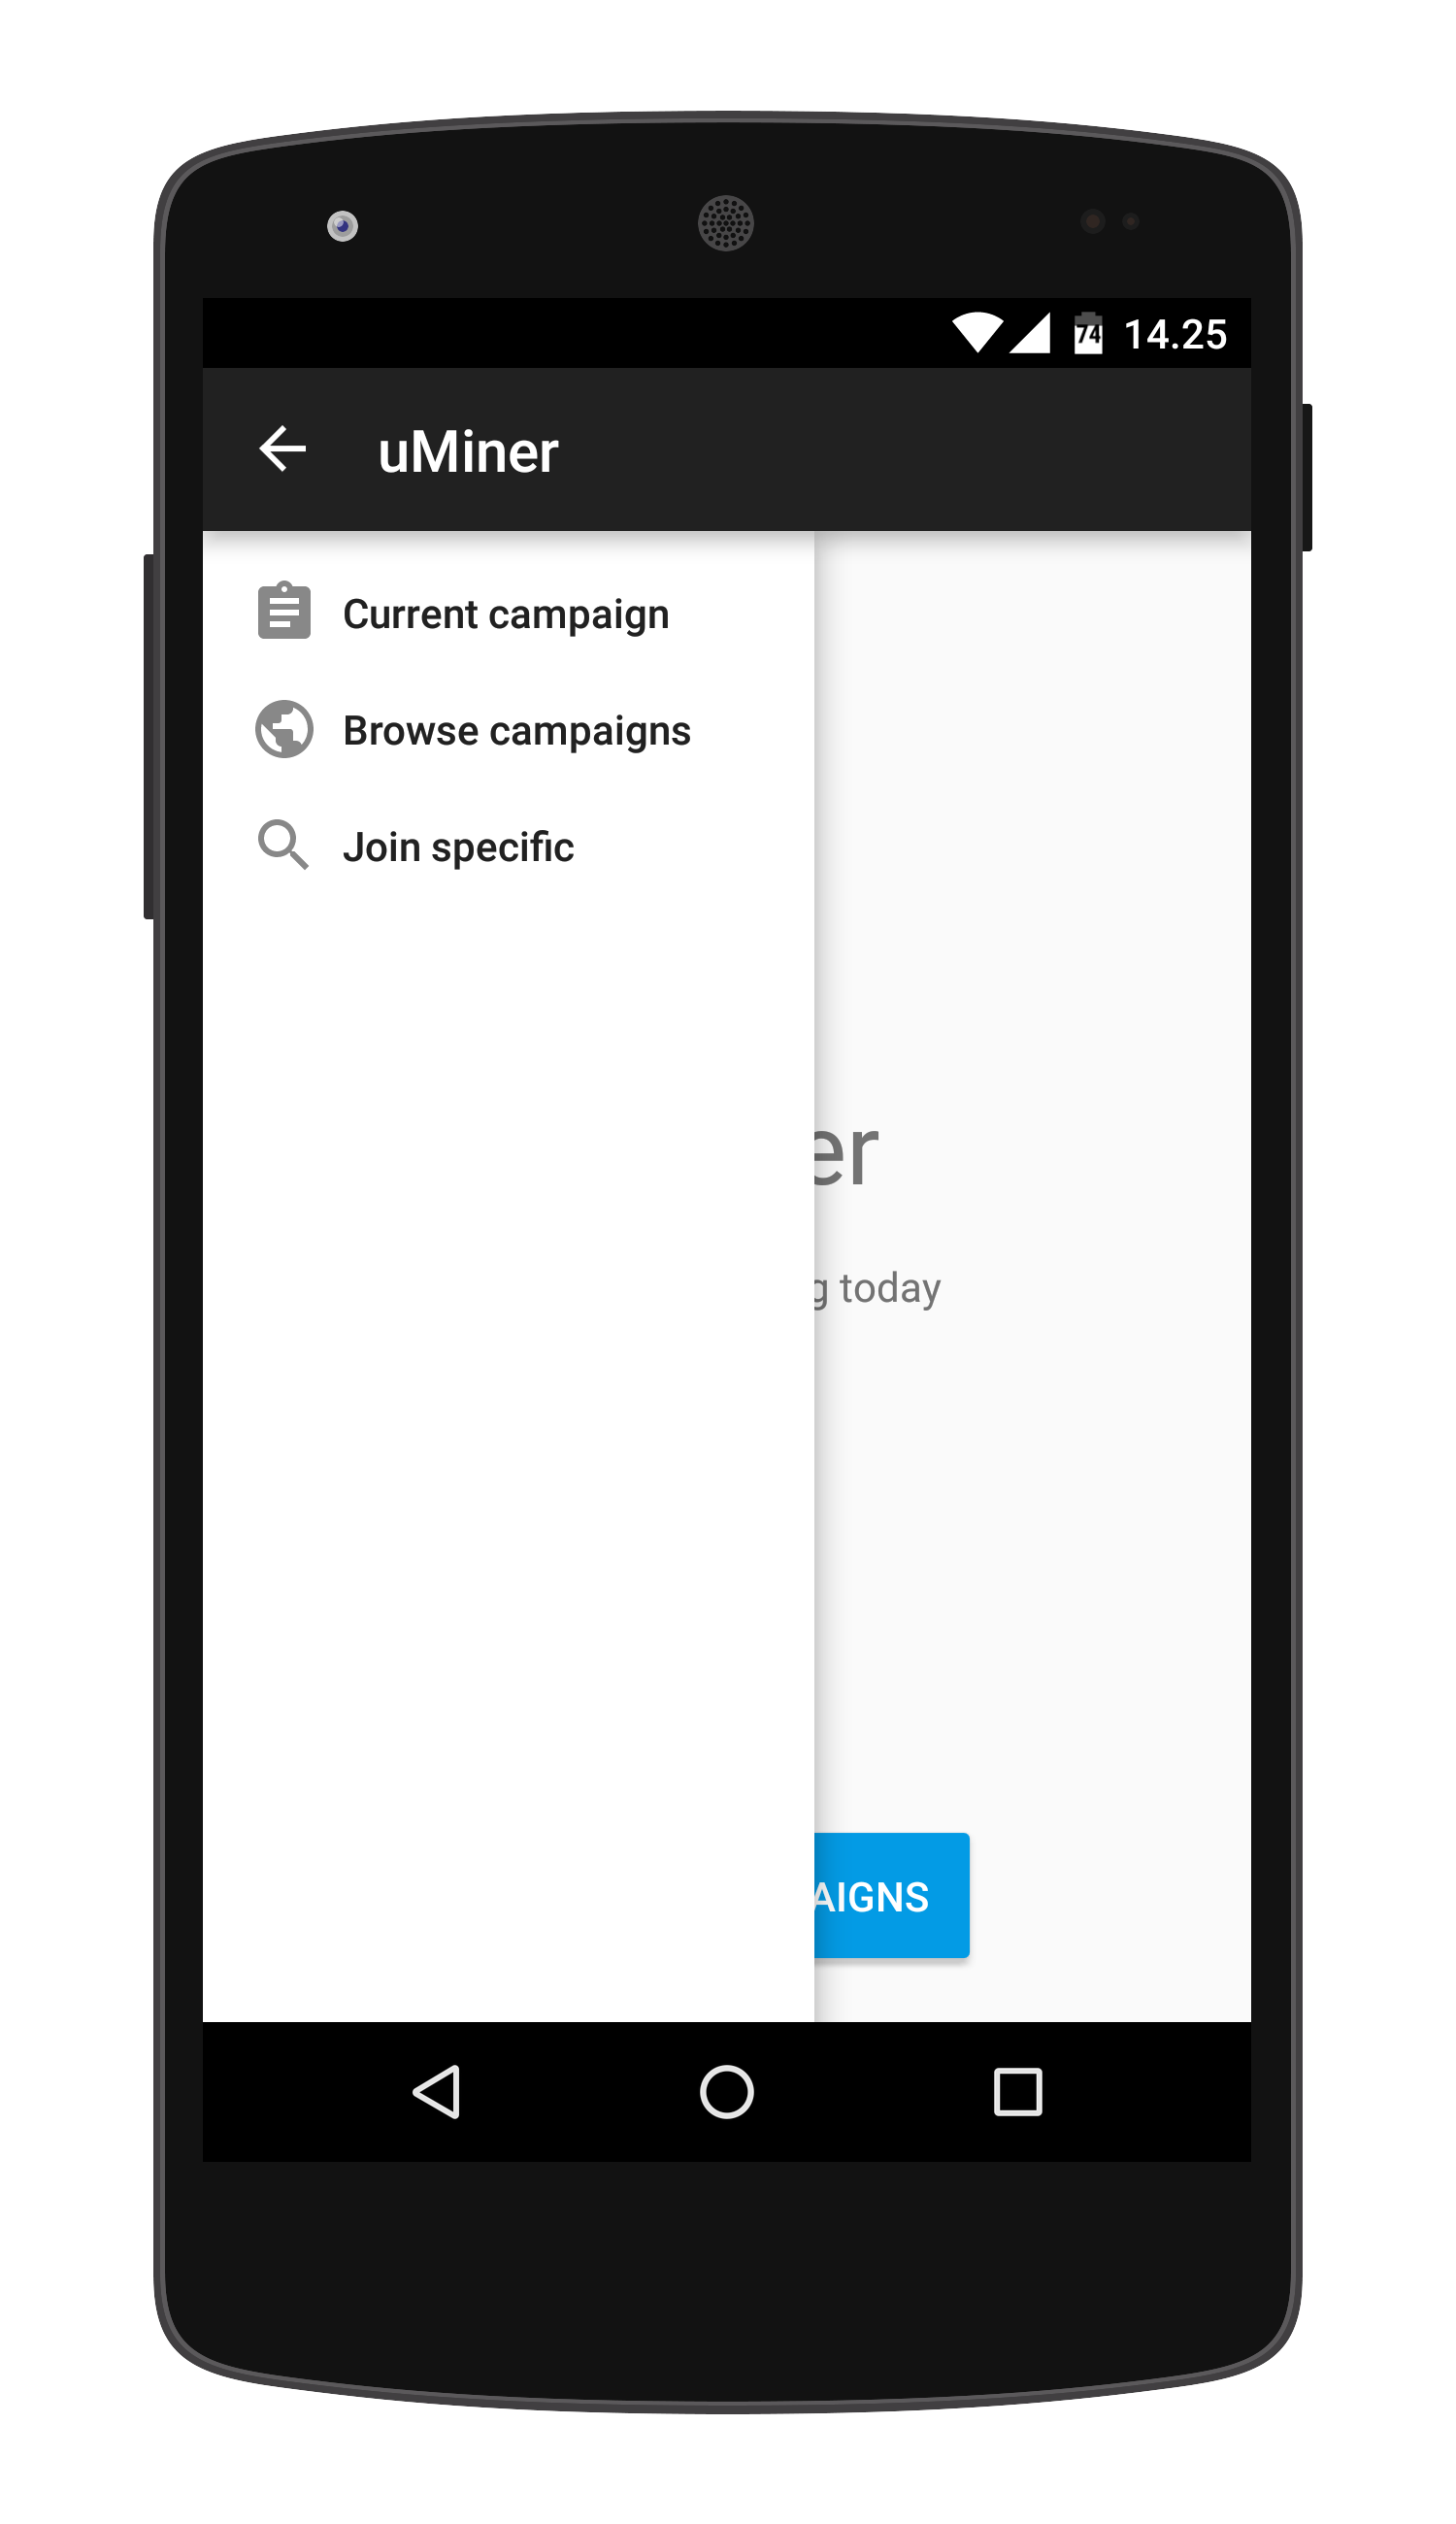
\includegraphics[width=.35\linewidth]{user_interfaces/client/client_drawer_menu_with_phone}
    \caption{Navigation through the application.}
    \label{fig:navigation}
\end{figure}
\FloatBarrier

\subsection{Browsing Campaigns}
\label{sub:browsing_campaigns}



 If participants want to contribute to a campaign, they may browse the publicly available campaigns, which can be done through the screen seen in \figref{fig:public_campaigns}. All the publicly available campaigns are listed here, each with its own entry displaying the title alongside the author of the campaign. If the participant wishes to learn more about one of the listed campaigns, he can press on that campaign and be redirected to a screen similar to the one seen in \figref{fig:campaign_specification}, where more detailed information about the selected campaign is shown. 
\\\\
We have for the implementation of the listing of campaigns utilized a design pattern called the \emph{view holder} design pattern \parencite{view_holder_pattern} together with an Android \mono{Adapter}. The \mono{Adapter} makes sure that we can reuse \mono{View} instances and thus prevents constant allocation and deallocation of \mono{View}s when the user is scrolling the list. Using the heap excessively is expensive in terms of CPU cycles in Java and triggers the garbage collector to run more than necessary \parencite{android_garbage_collection}. We would thus like to minimize use of the heap. Reusing \mono{View}s helps reduce battery consumption and should improve the general performance perceived by users and prevent stuttering in the graphical interface. Alongside the \emph{view holder} pattern, only the data, which is strictly necessary for displaying the list is downloaded for this screen. More detailed information is fetched when needed by other screens.

% Publicly available campaigns
\begin{figure}[!htbp]
    \begin{subfigure}[!t]{.48\textwidth}
        \centering
        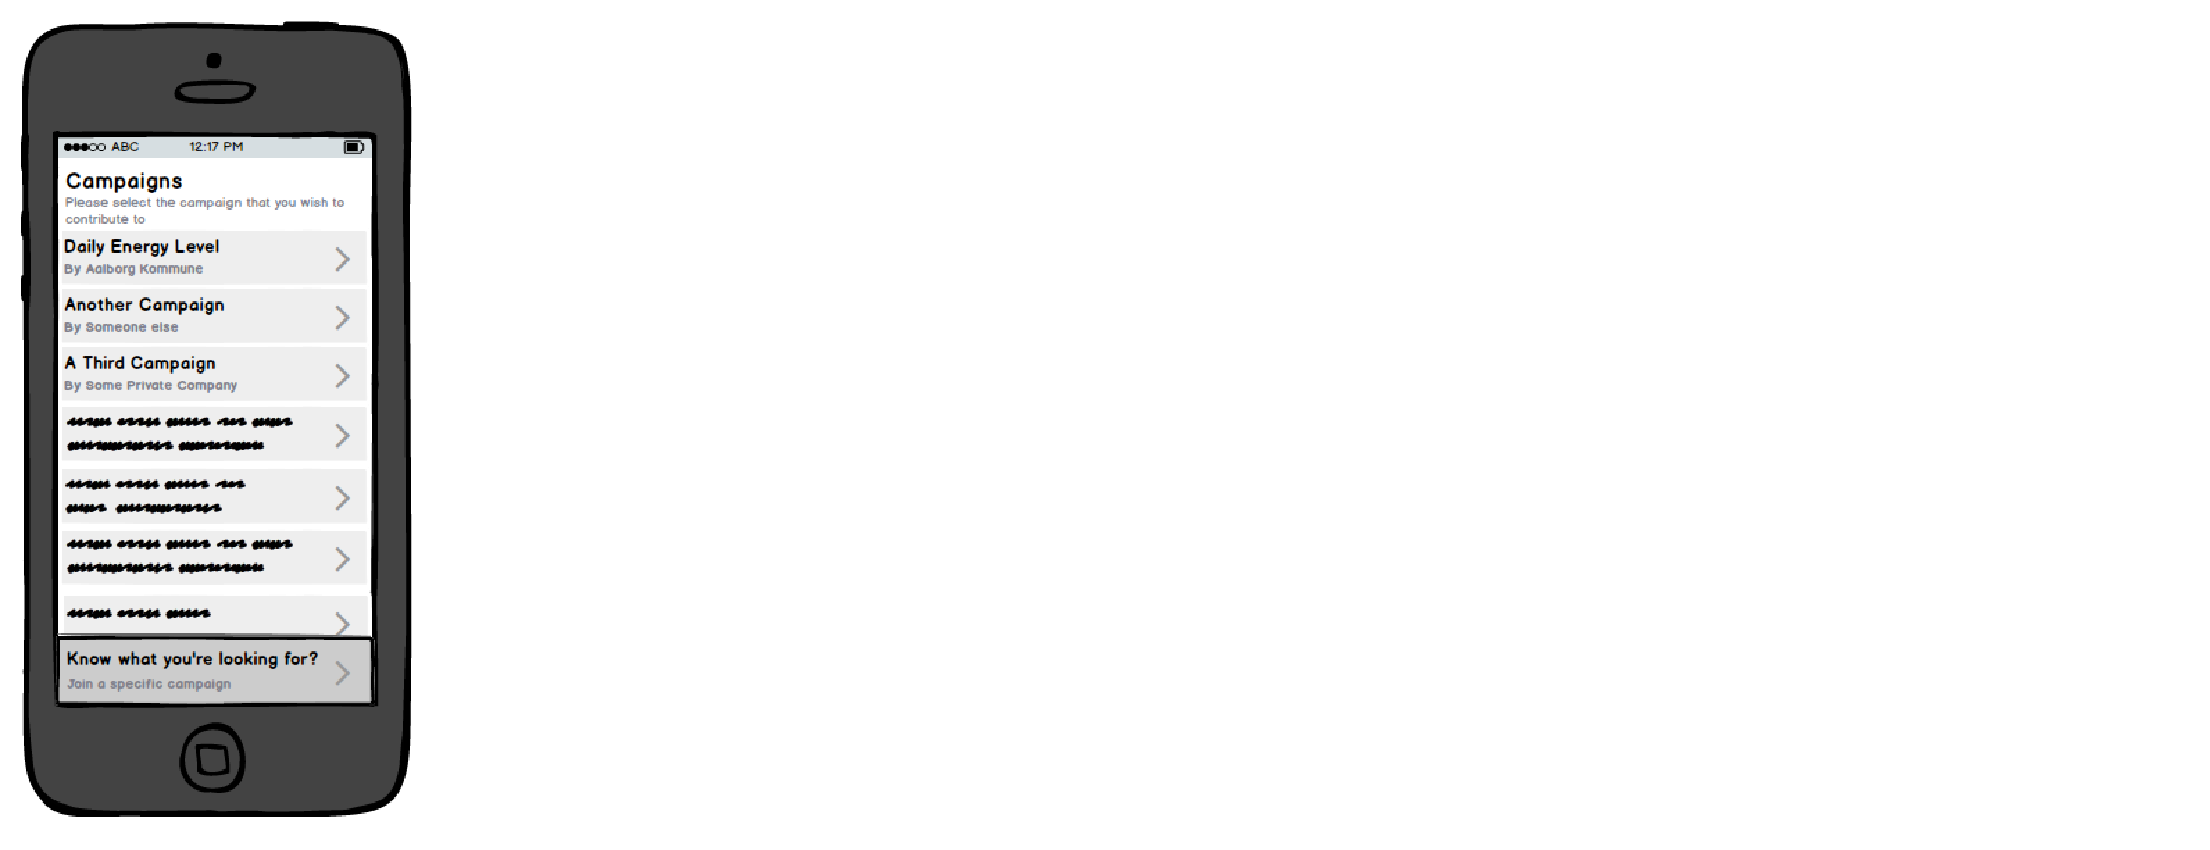
\includegraphics[width=.7\linewidth]{mockups/campaigns_list}
        \caption{Mockup of the browsing screen.}
        \label{fig:mockup_public_campaigns}
    \end{subfigure}%
    \begin{subfigure}[!t]{.52\textwidth}
        \centering
        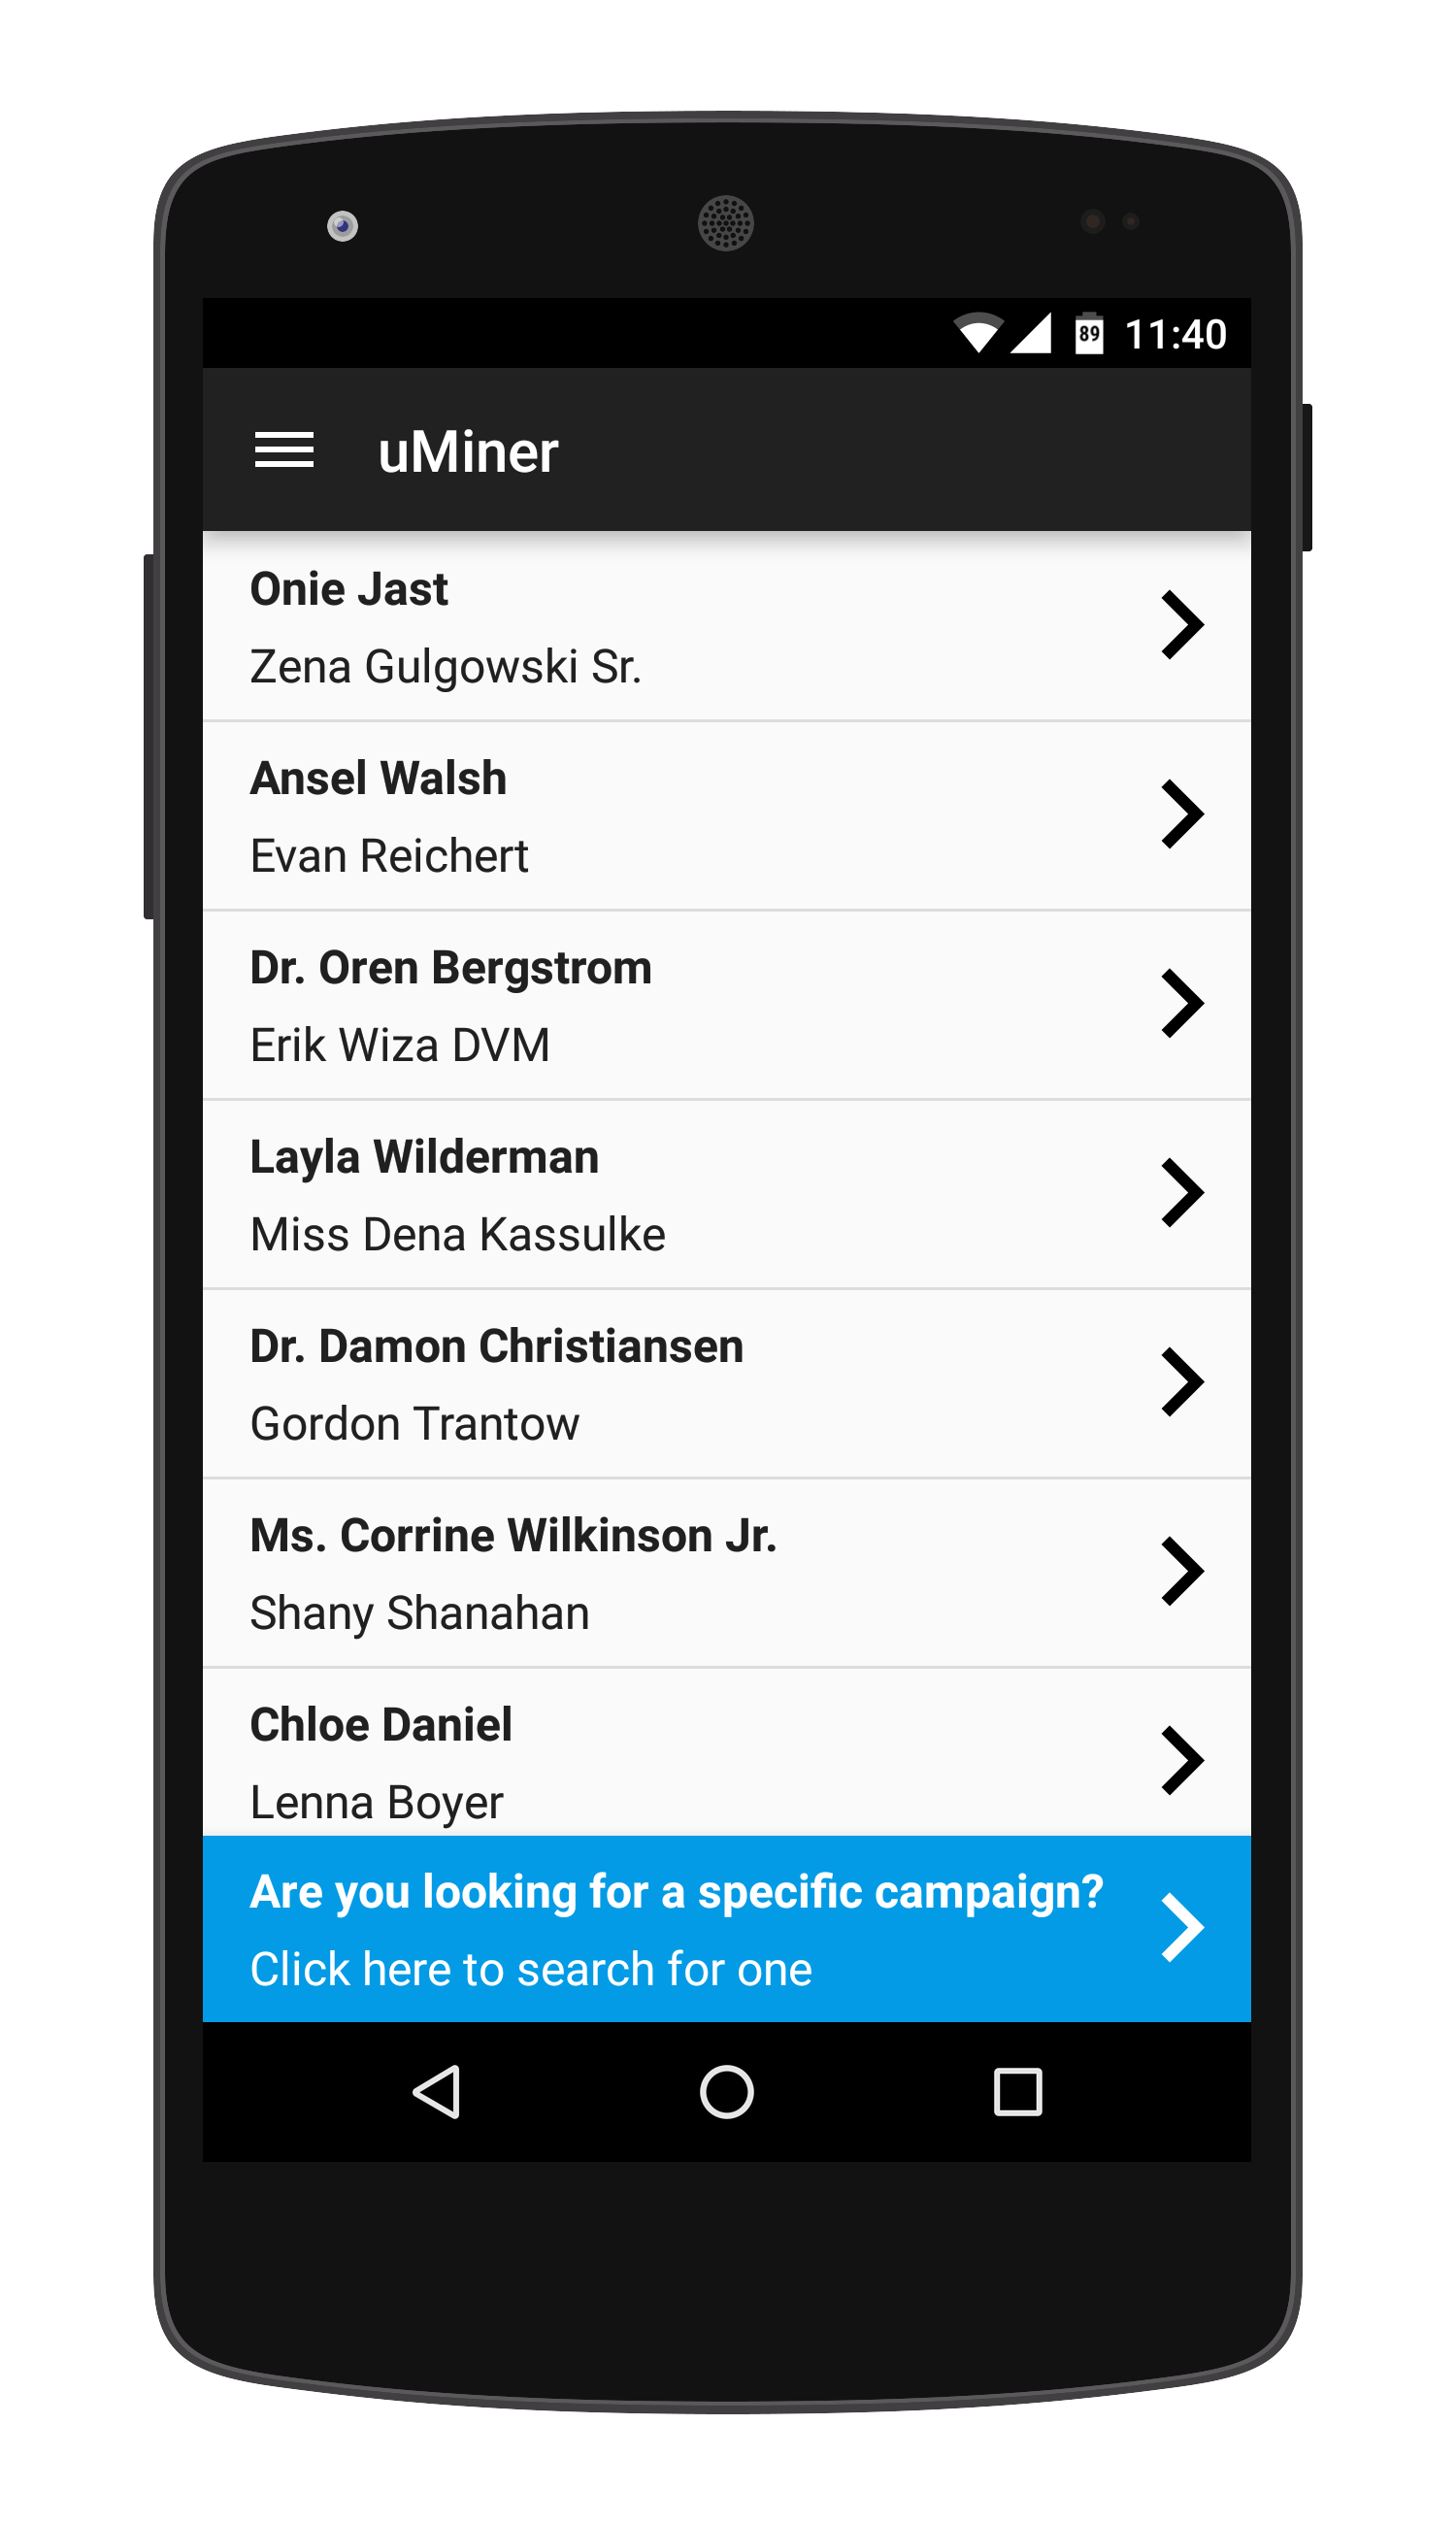
\includegraphics[width=.73\linewidth]{user_interfaces/client/client_public_campaigns_with_phone}
        \caption{Implementation of the browsing screen.}
        \label{fig:implementation_public_campaigns}
    \end{subfigure}
    \caption{Mockup and implementation of browsing campaigns.}
    \label{fig:public_campaigns}
\end{figure}
\FloatBarrier

The participant also has the opportunity to join a specific campaign, when browsing the public ones, by pressing the blue area in the bottom, which will always be visible regardless of how far the participant scroll in the list. If the area is pressed, the participant will be redirected to the screen showed in \figref{fig:specific_campaign}. Participants can here enter a unique campaign identifier, if they have been given one by a customer. The participant will, upon entering an identifier, be redirected to a screen similar to the one seen in \figref{fig:campaign_specification} if the specified identifier corresponds to a campaign. If not, the participant will be notified that the entered campaign identifier is invalid. 

% Search for a campaign through a campaign identifier
\begin{figure}[!htbp]
    \begin{subfigure}[!t]{.48\textwidth}
        \centering
        
\includegraphics[width=.7\linewidth]{mockups/join_specific_campaign}
        \caption{Mockup for the searching.}
        \label{fig:mockup_specific_campaign}
    \end{subfigure}%
    \begin{subfigure}[!t]{.52\textwidth}
        \centering
        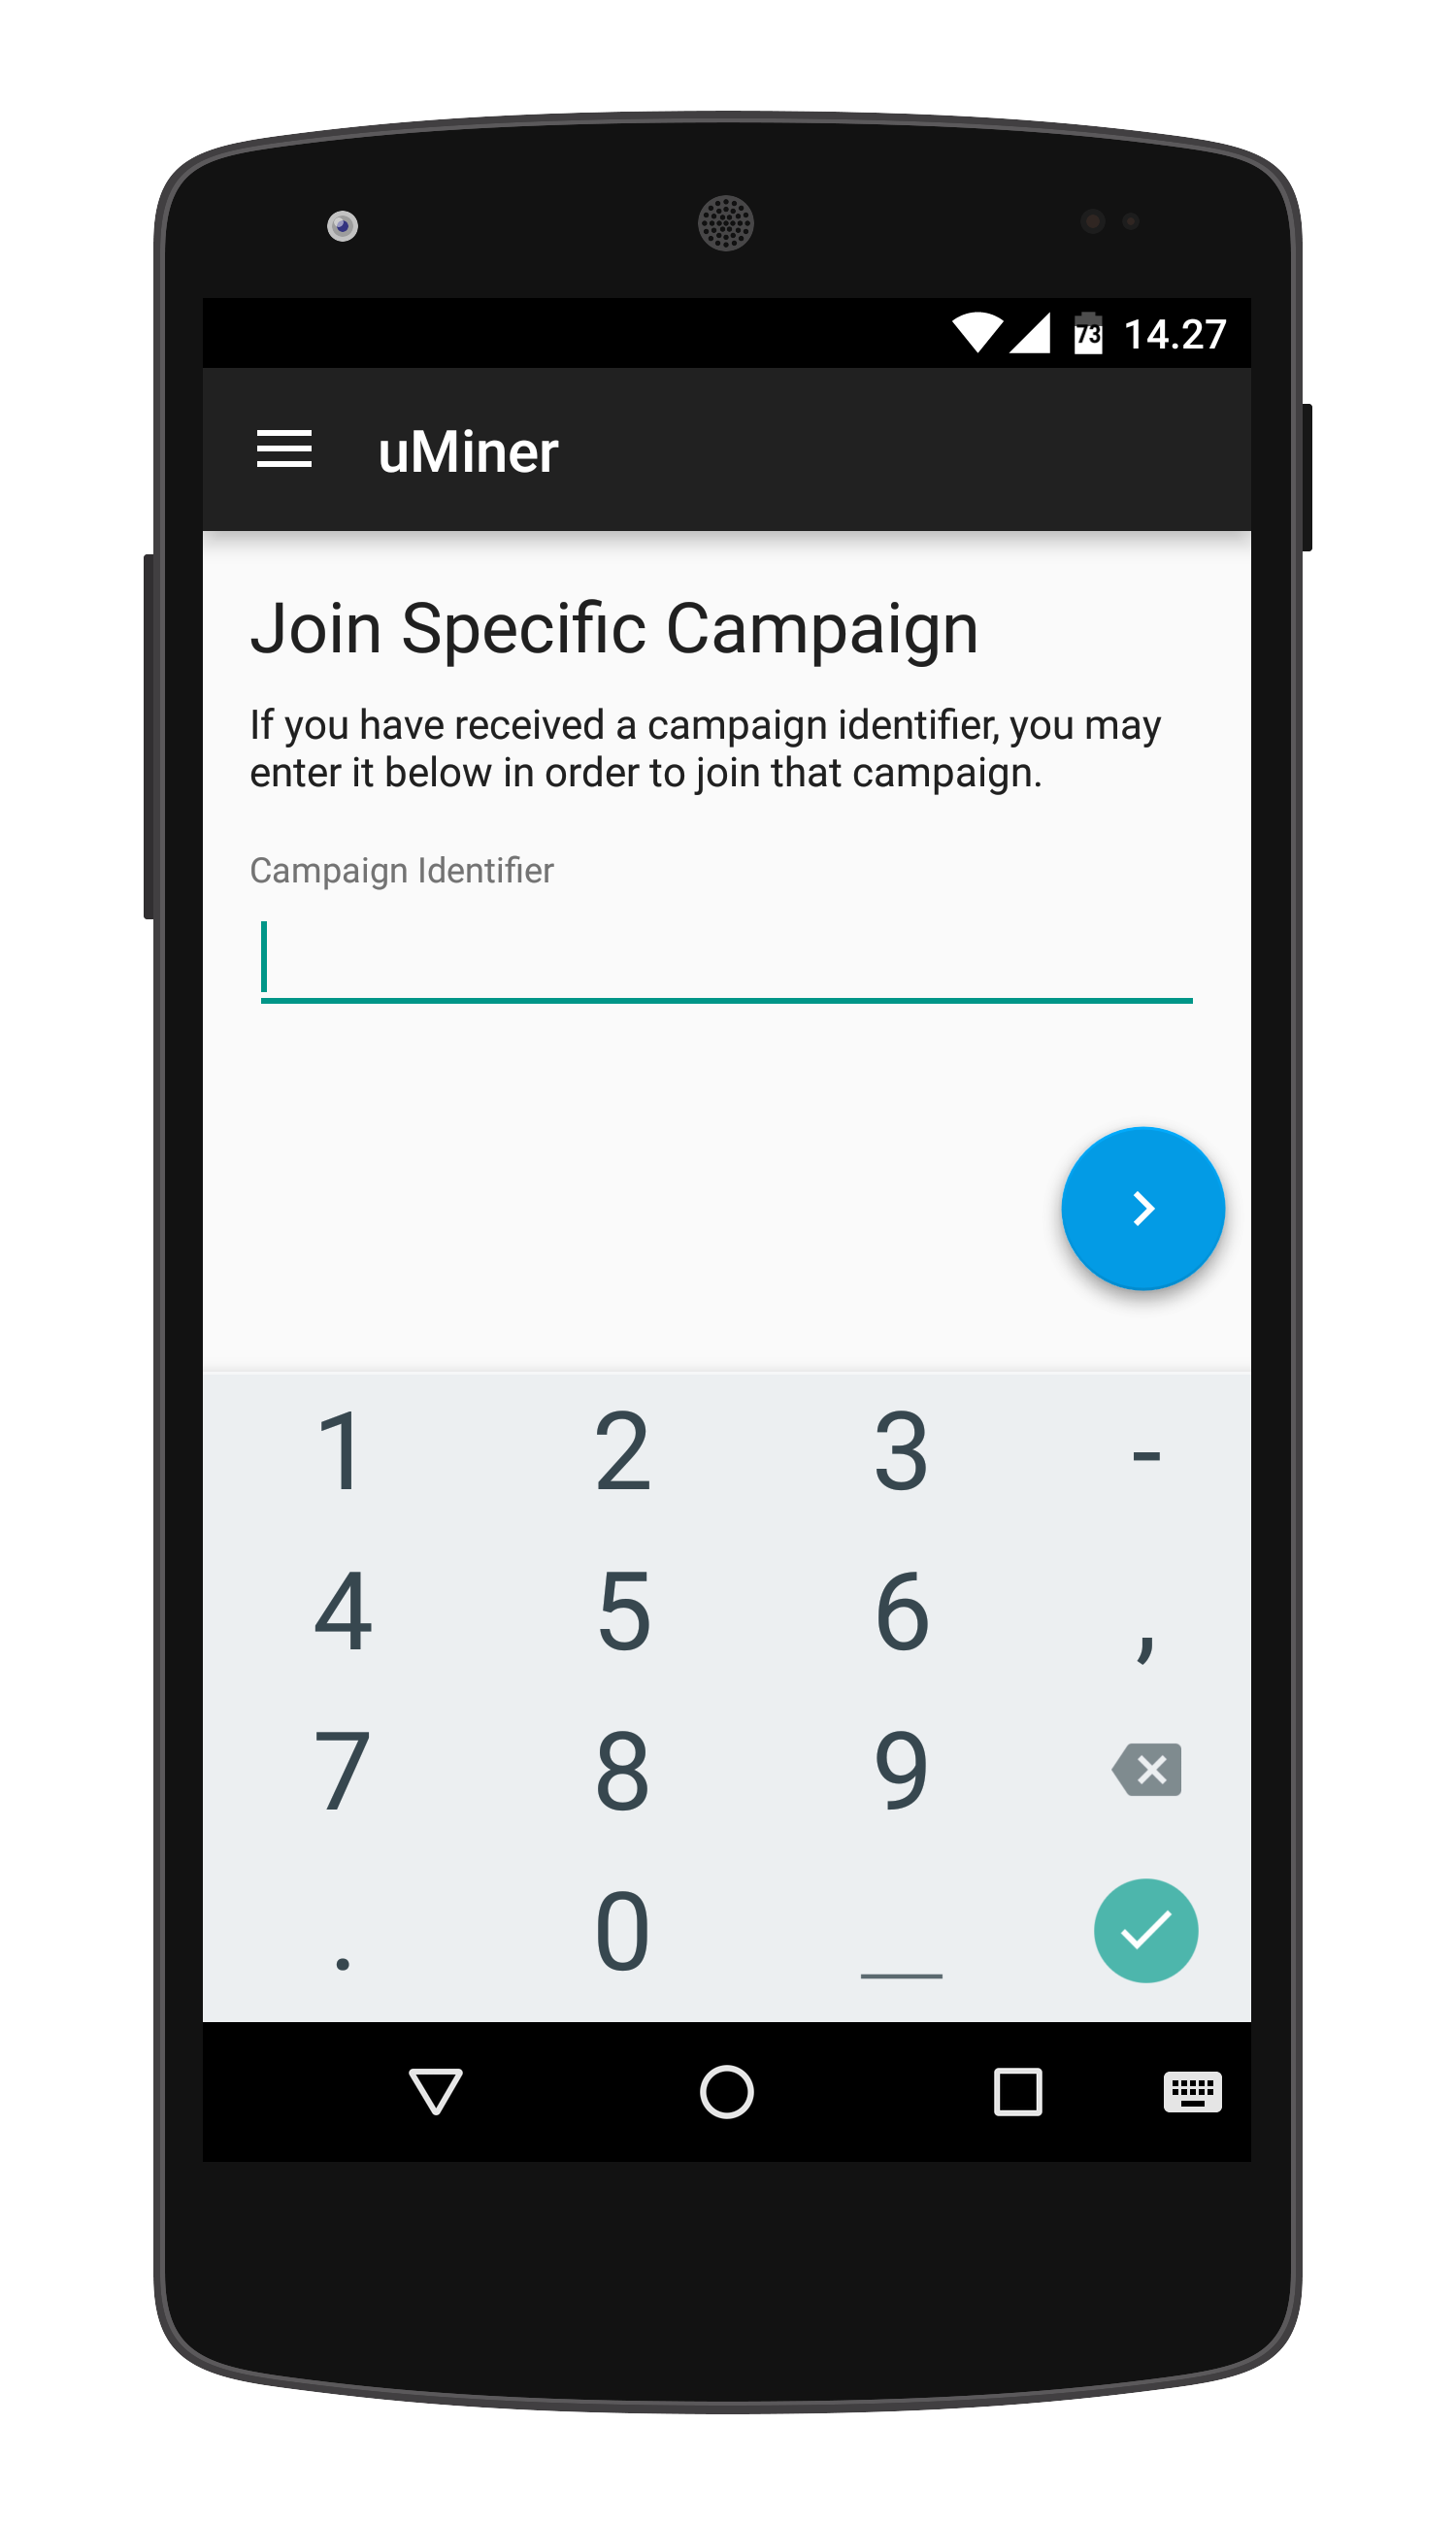
\includegraphics[width=.73\linewidth]{user_interfaces/client/client_join_specific_campaign_with_phone}
        \caption{Implementation for the searching.}
        \label{fig:implementation_specific_campaign}
    \end{subfigure}
    \caption{Mockup and Implementation for searching for a specific campaign using a campaign identifier.}
    \label{fig:specific_campaign}
\end{figure}
\FloatBarrier

The mobile application currently only supports scrolling through the list of public campaigns to find a campaign. One could imagine that at some point in time the amount of campaigns would increase to a number, where it would be infeasible to scroll through. This could be solved by utilizing filtering or querying of campaigns. If this were to be implemented it would be beneficial to do this on the server, such that the device should not download all the information needed to process such queries or filters. Throughout the project period, we have thought of a number of different ways of allowing the participants to find and join campaigns, which could prove to be nice additions to the system, but have not been implemented yet.

\begin{description}
    \item[Quick Response (QR) Codes] could be utilized to give participants an easy way of subscribing to campaigns, by scanning a QR code. Customers would be able to distribute these QR codes through both digital and printed media. Furthermore, QR codes might be more easily relatable for participants, since they might be familiar with the concept from other domains.

    \item[Specific search criteria] might help participants to find exactly what they want to contribute to. Participants might only be willing to contribute to campaigns with a scientific purpose, or campaigns that have next to no impact on battery life. Other criteria might be: limited amount of questions in questionnaires, or none at all. Additionally, some participants might not be willing to contribute to campaigns with specific sensors, e.g. GPS, so the possibility of filtering campaigns by different sensors might also be desirable.

    \item[Prizes and other motivational factors] are not present in the current state of the system. However, if they were to be introduced, they would potentially have a big impact on which campaigns gets contributed to. This means that the application could assist customers in getting more participants for their campaigns by displaying information regarding the prizes that customers provide to contributing participants. One could also imagine that participants could filter campaigns depending on whether they provide a reward or not.
\end{description} 

\subsection{Contributing to Campaigns}
\label{sub:contributing_to_campaigns}

To contribute to a specific campaign, participants must firstly find a campaign that they want to contribute to. This can be done through the campaign browser, previously shown in \figref{fig:public_campaigns}, or entering a unique identifier in the join specific campaign screen, previously shown in \figref{fig:specific_campaign}. The participants must then navigate to a campaign specification screen, similar to the one seen in \figref{fig:campaign_specification}. 
\\\\
After a participant has found a campaign that he is willing to contribute to, he will find himself on an overview of the information related to the campaign on a screen similar to the one seen in \figref{fig:campaign_specification}. After reviewing this information, the participant can decide if he wants to contribute by subscribing to the campaign, which will be done by pressing the green subscribe button. This will signal the background service to start the collection of snapshots as described in \secref{sub:background_sensor_service_snapshot_generation_and_upload}.

% Campaign specification
\begin{figure}[!htbp]
    \begin{subfigure}[!t]{.48\textwidth}
        \centering
        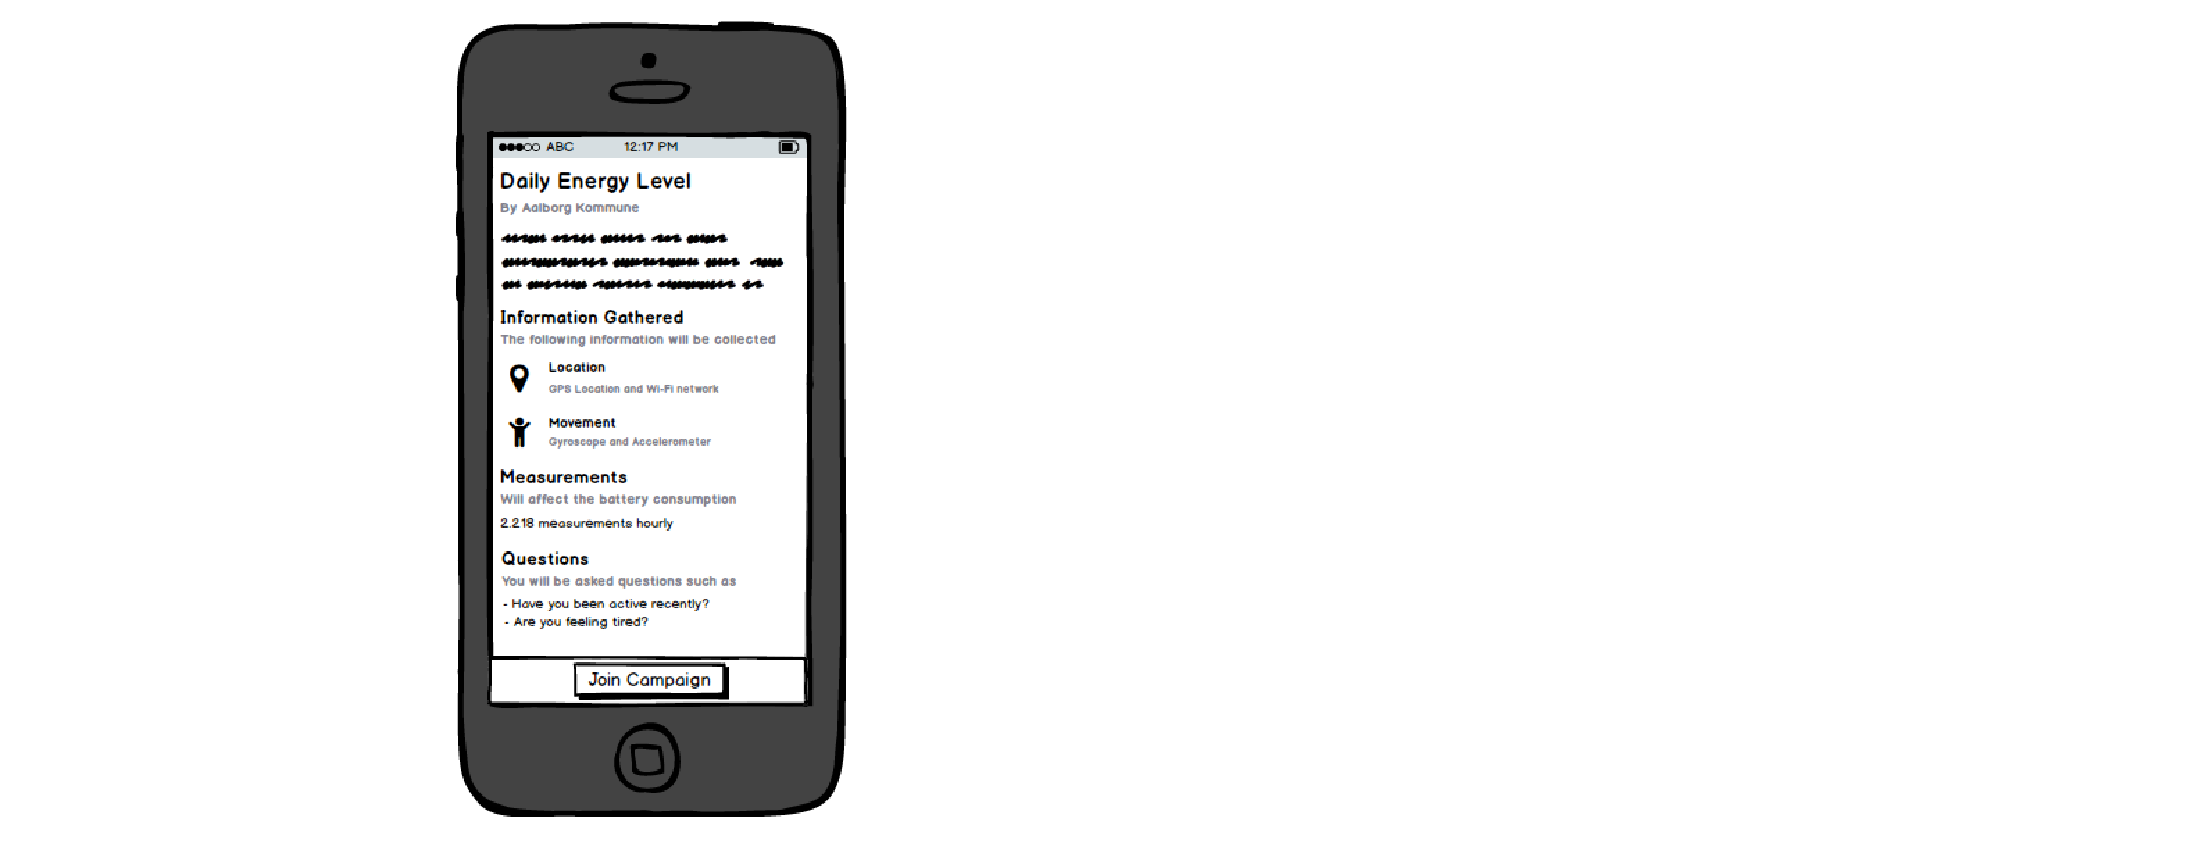
\includegraphics[width=.7\linewidth]{mockups/campaign_specification}
        \caption{Mockup of the specification screen.}
        \label{fig:mockup_campaign_specification}
    \end{subfigure}%
    \begin{subfigure}[!t]{.52\textwidth}
        \centering
        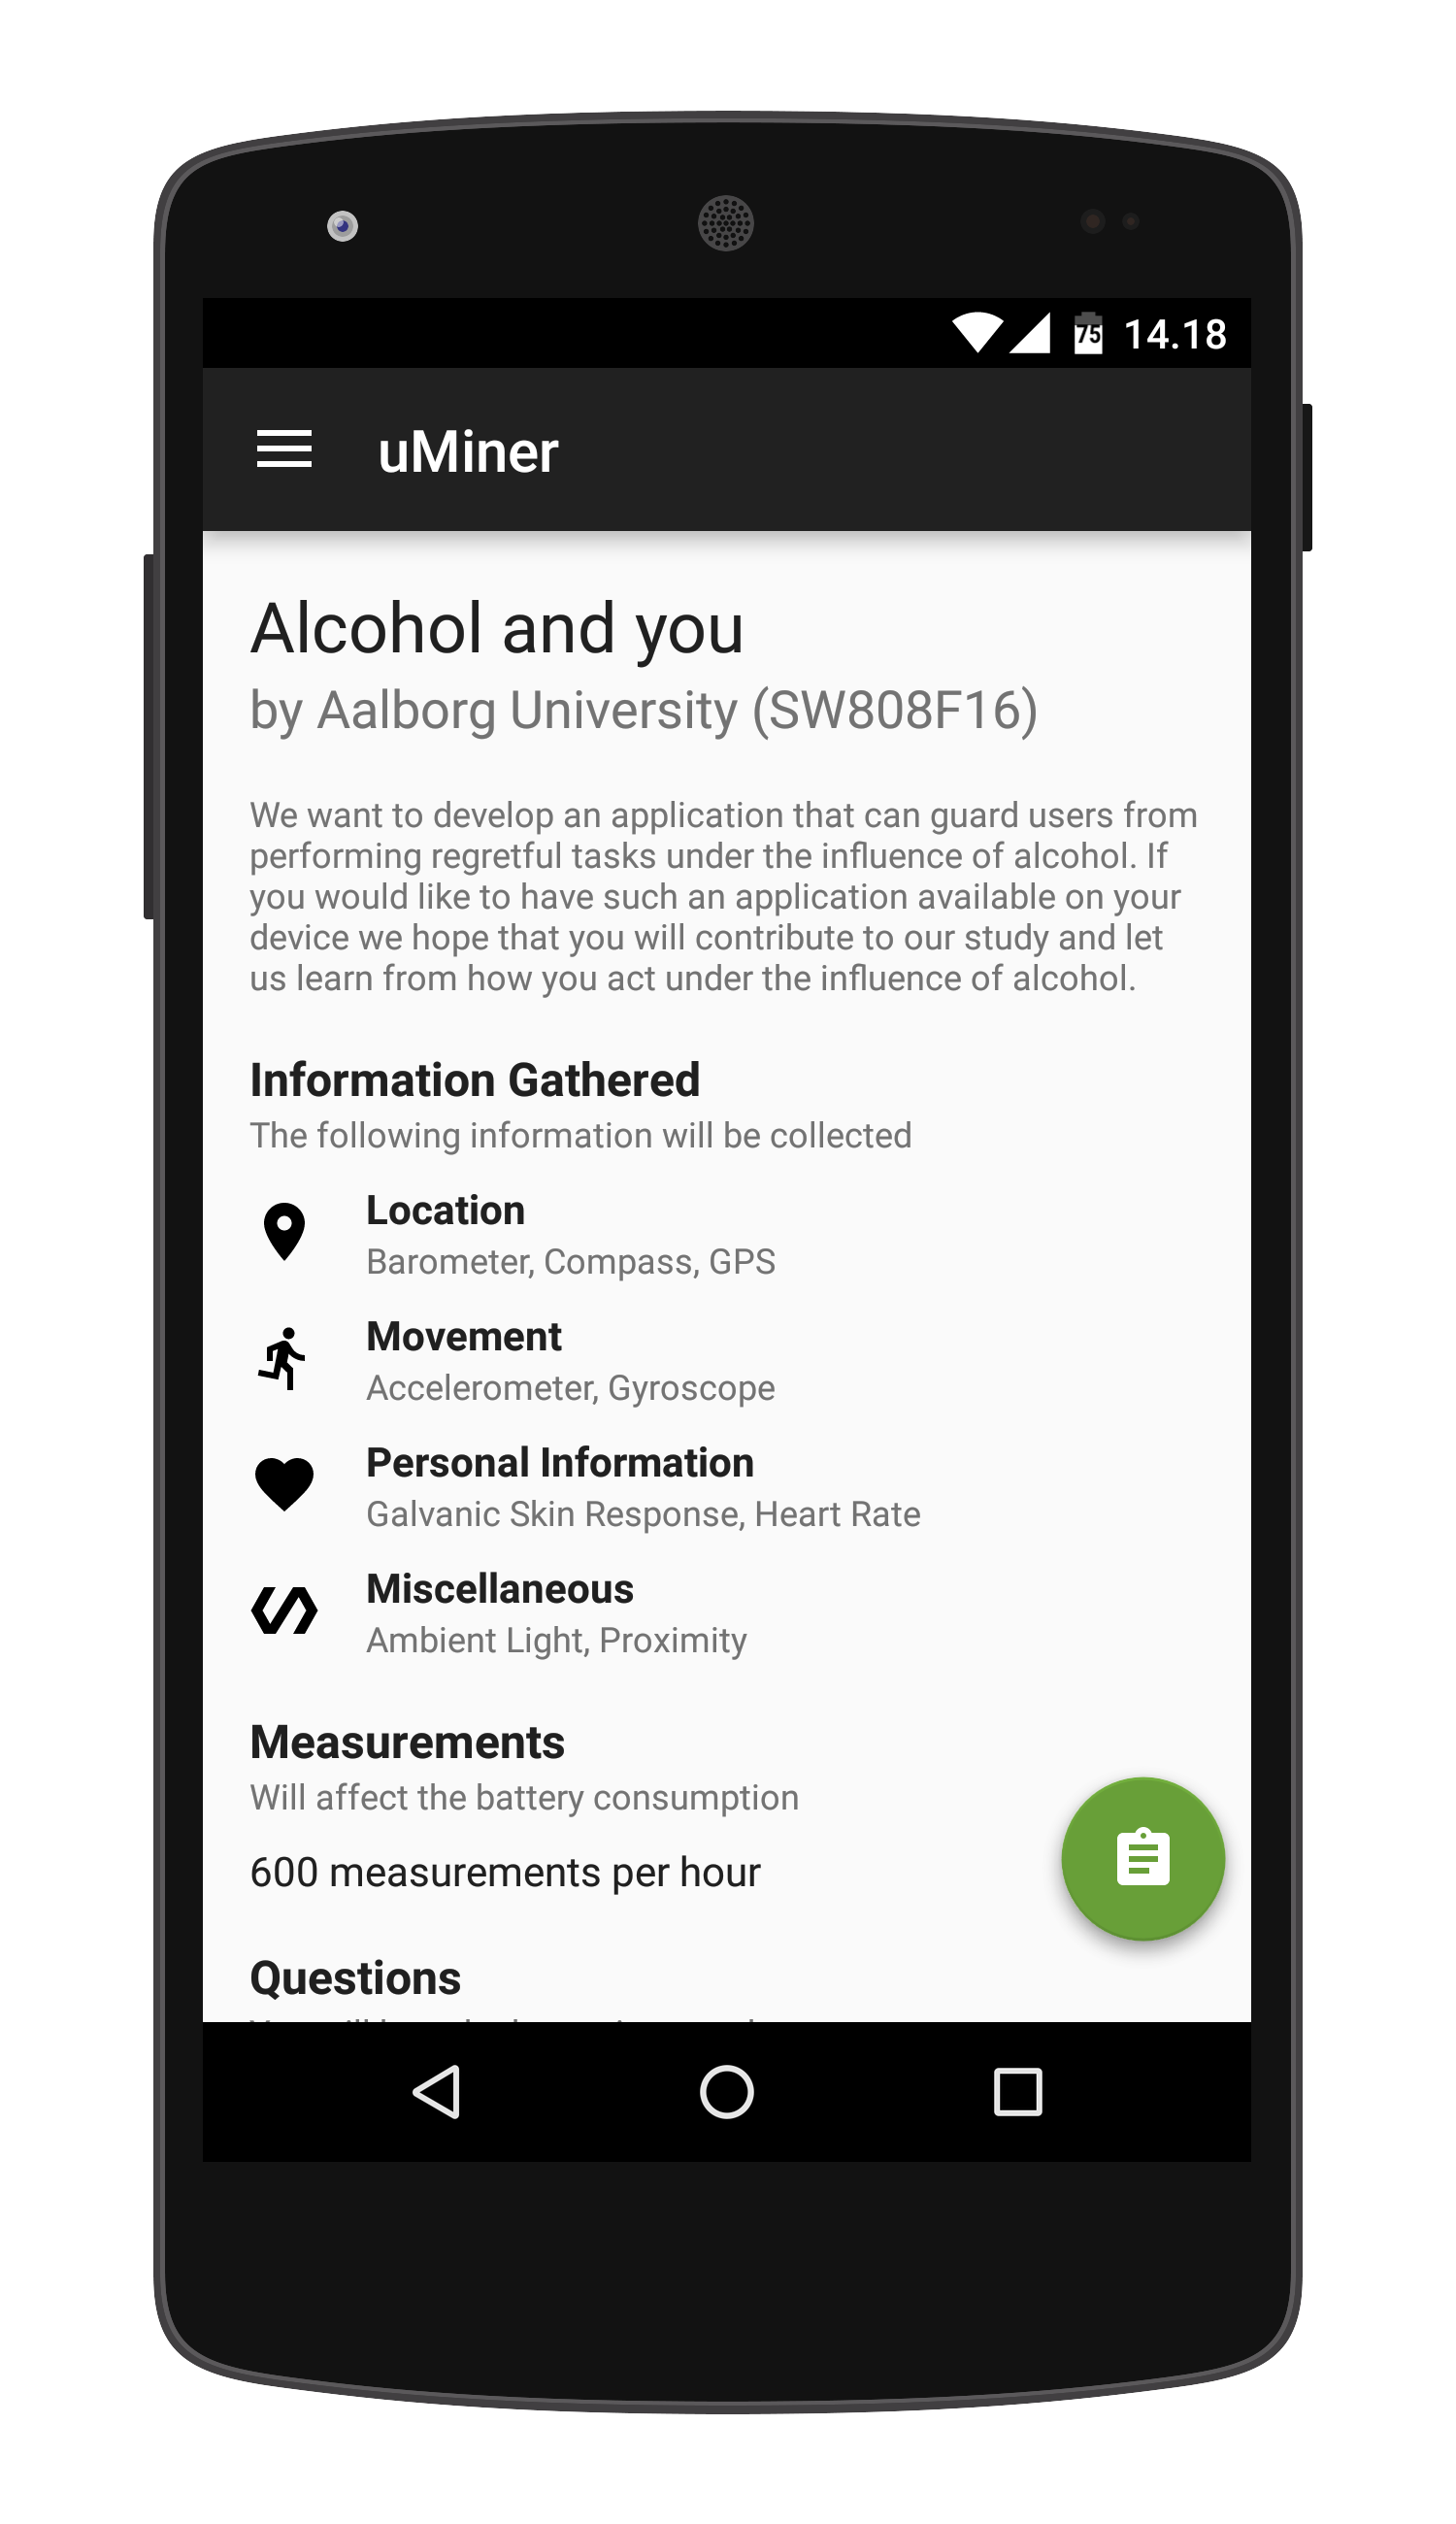
\includegraphics[width=.73\linewidth]{user_interfaces/client/client_campaign_specification2_with_phone}
        \caption{Implementation of the specification screen.}
        \label{fig:implementation_campaign_specification}
    \end{subfigure}
    \caption{Mockup and implementation of the specification screen for a campaign.}
    \label{fig:campaign_specification}
\end{figure}
\FloatBarrier

If for any reason, a participant no longer wishes to contribute to a campaign, he can navigate to the specification for the given campaign. This time, the otherwise green subscribe button will instead be a red unsubscribe button, as seen in \figref{fig:leave_campaign_no_dialog}. Pressing this button, will prompt the participant with a confirmation dialog, as seen in \figref{fig:leave_campaign_dialog}. If the participant confirms the action, by pressing yes, the background sensor service is signaled to stop generating snapshots. However, the snapshot currently being generated will complete and be uploaded to the server. This happens because the service (described in \secref{sec:background_sensor_service}) that starts the sensor gathering does not have a hook on the threads that produces output from sensors, and for that reason it is, in the current state of uMiner, not possible to stop the gathering immediately.

% Leave campaign and dialog
\begin{figure}[!htbp]
    \begin{subfigure}[!t]{.50\textwidth}
        \centering
        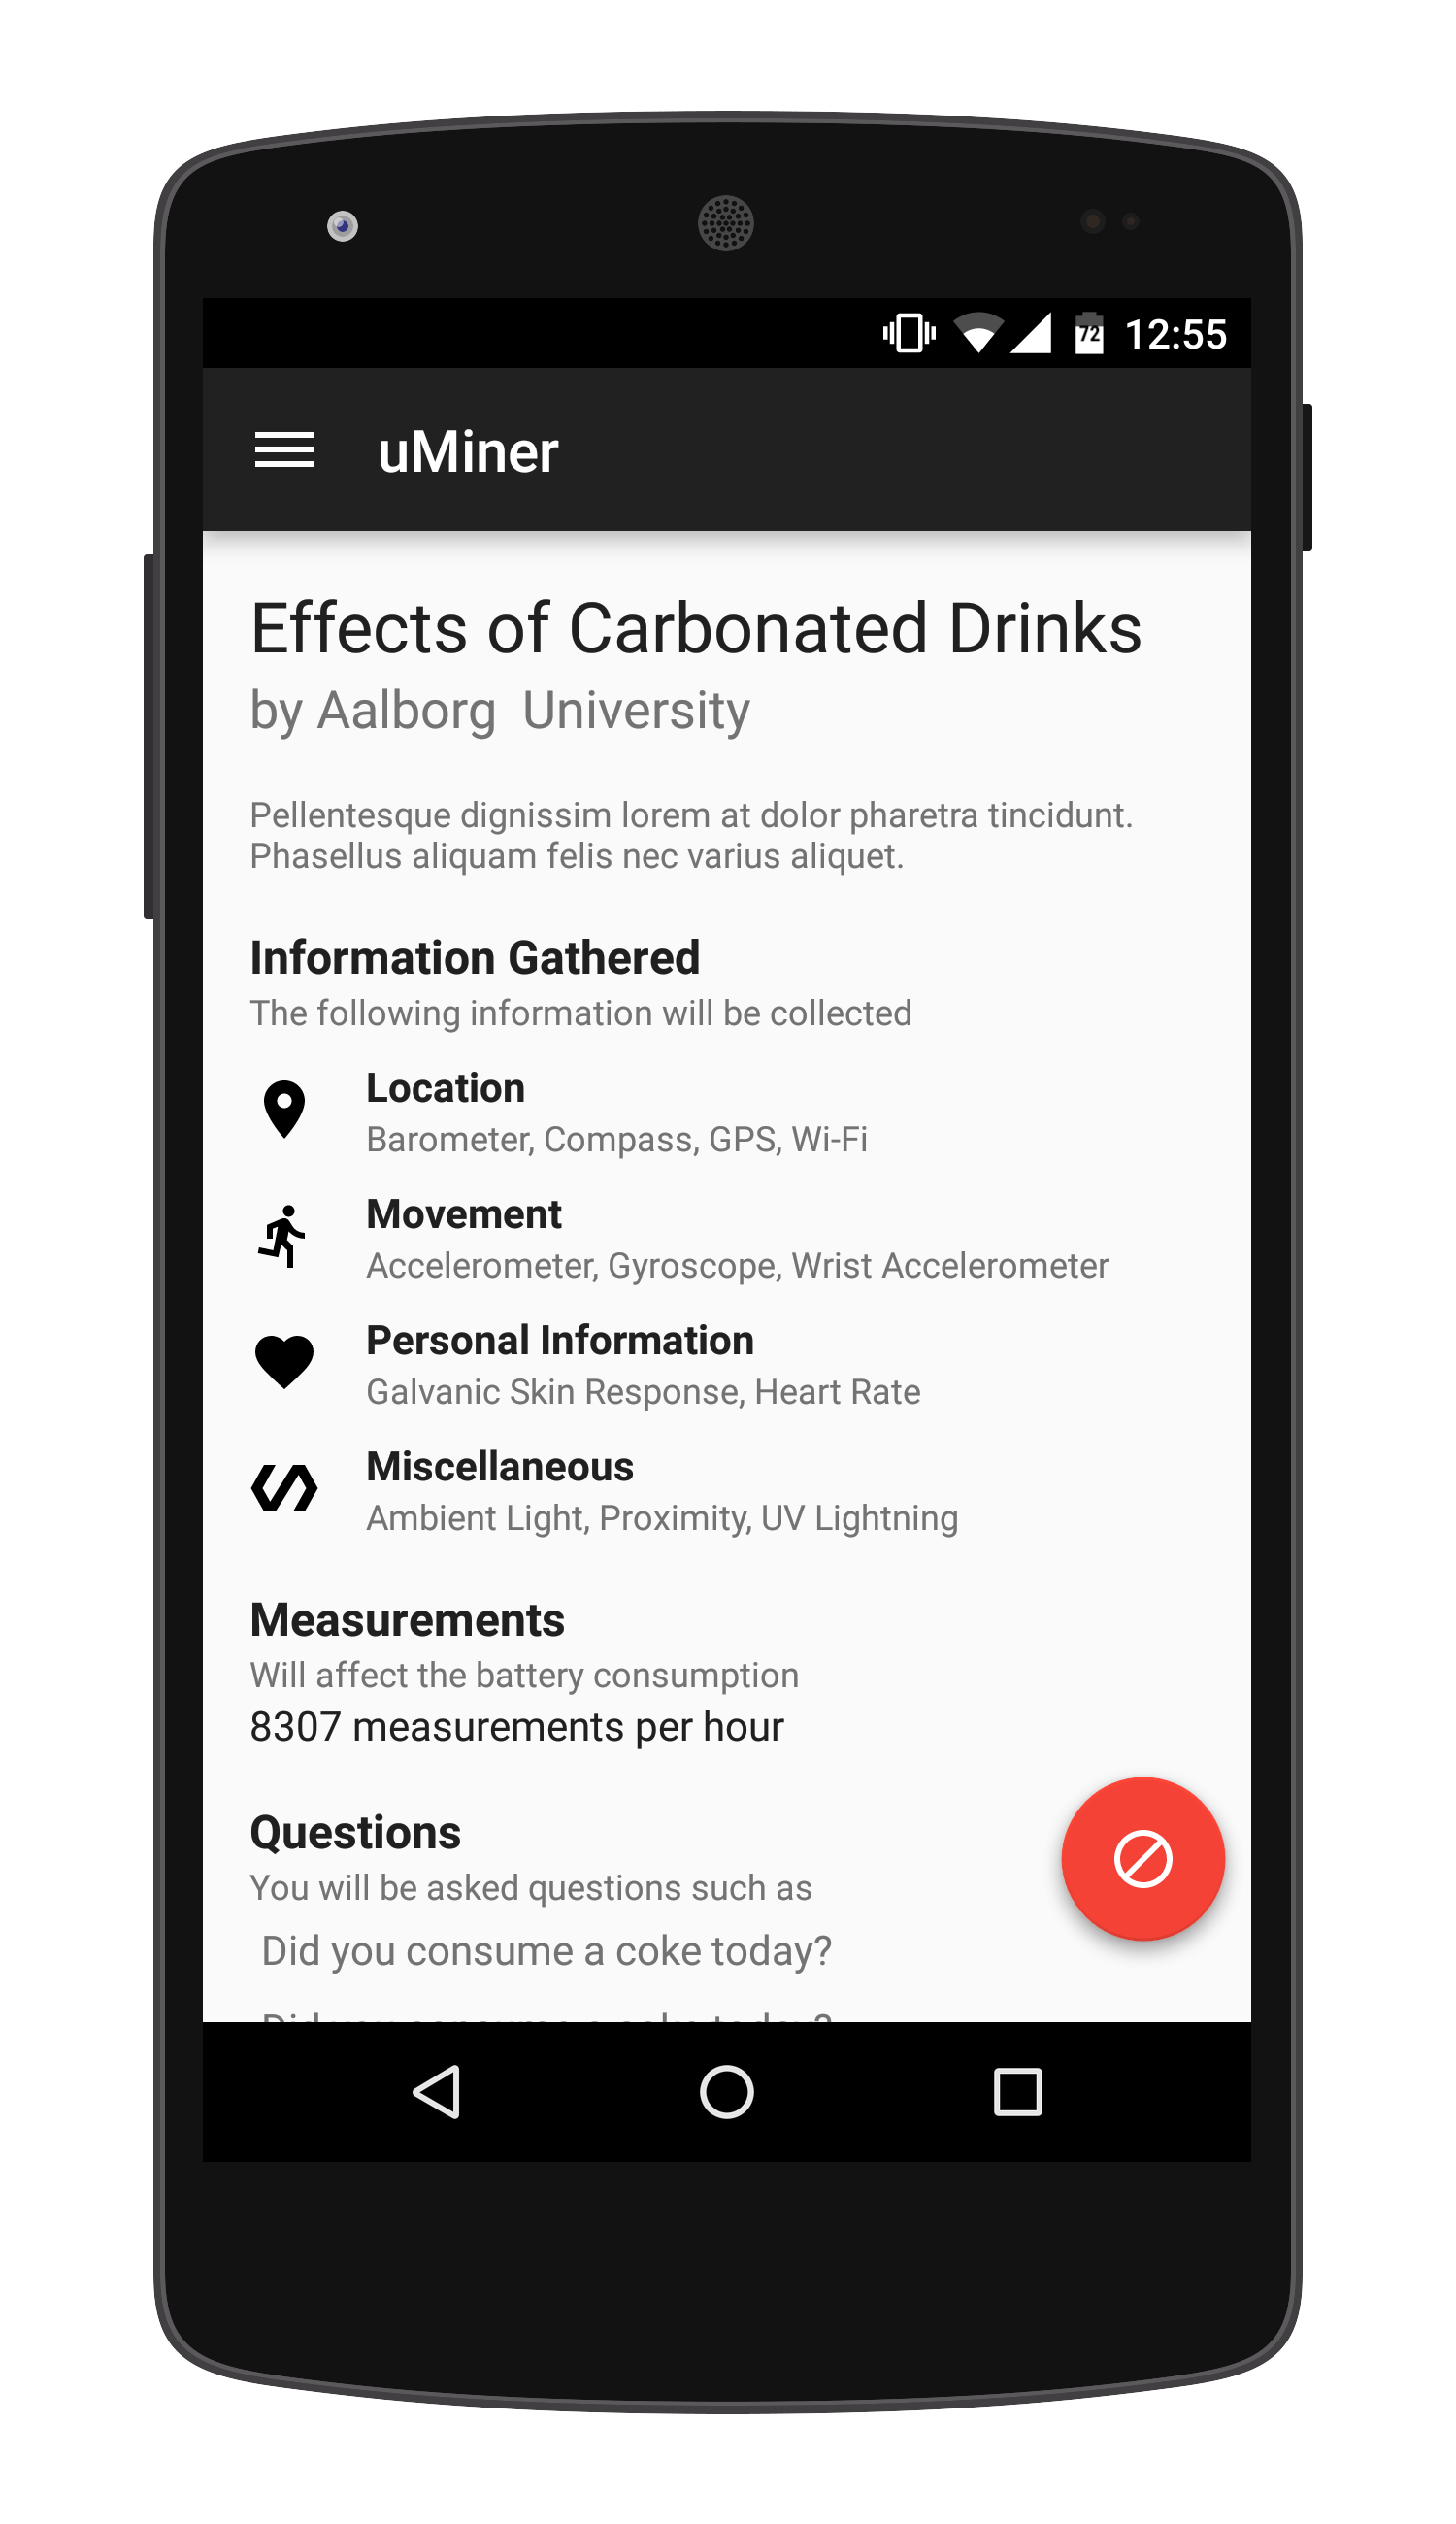
\includegraphics[width=.73\linewidth]{user_interfaces/client/client_leave_campaign_no_dialog_with_phone}
        \caption{Specification screen with an unsubscribe \\\hspace{\textwidth}button.}
        \label{fig:leave_campaign_no_dialog}
    \end{subfigure}%
    \begin{subfigure}[!t]{.50\textwidth}
        \centering
        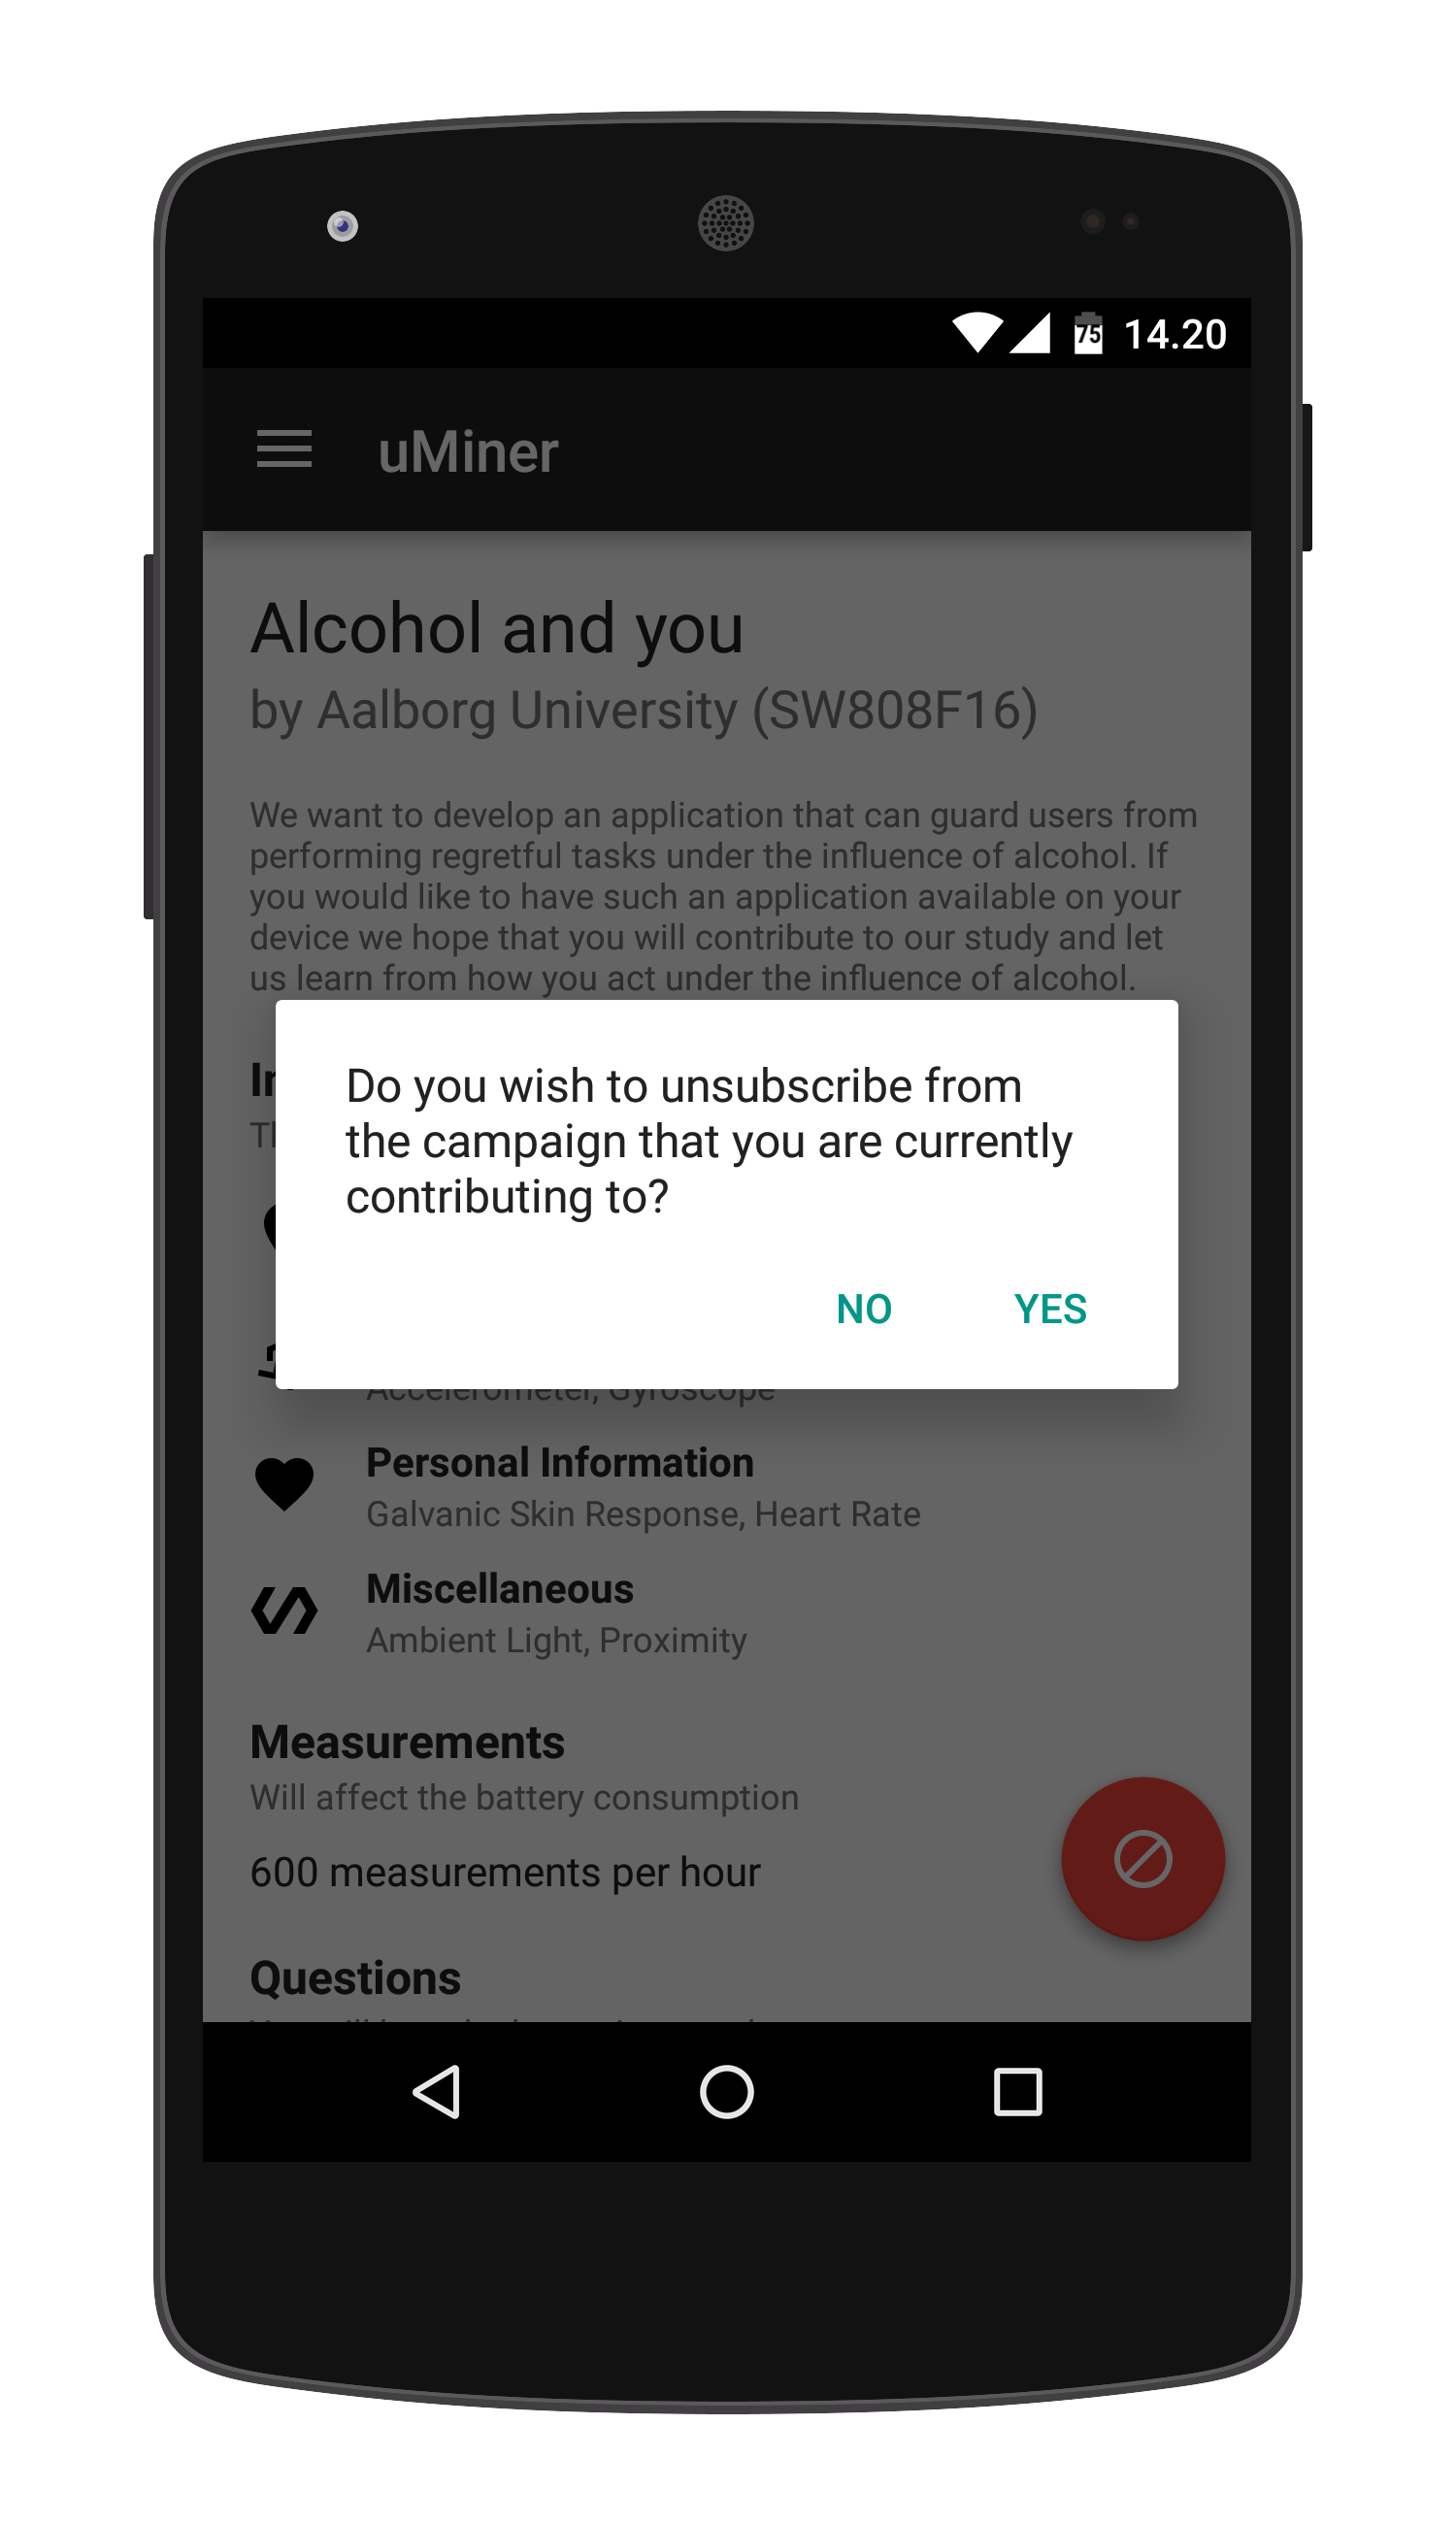
\includegraphics[width=.73\linewidth]{user_interfaces/client/client_leave_campaign_with_phone}
        \caption{Confirmation dialog triggered by pressing the unsubscribe button.}
        \label{fig:leave_campaign_dialog}
    \end{subfigure}
    \caption{Specification screen of a campaign when a participant has joined it.}
    \label{fig:leave_campaign}
\end{figure}
\FloatBarrier

\subsection{Answering Questionnaires}
\label{sub:answering_questionnaired}
% This complies with the way we intended the system to work regarding the participatory sensing as described in \secref{sec:human_activity_recognition}\todo{er det her godt nok?}.
A participant will be requested to answer questionnaires, if required by a campaign subscribed to by participant's device. These request can occur at any time, even at times where the participant is not actively using uMiner. We have chosen to use Android notifications \parencite{android_notifications} to facilitate these request to participants. A notification will then pop-up when a participant should answer questionnaires, as can be seen in \figref{fig:answering_questionnaire_notification}. One benefit of using Android notifications is, that it allows participants some degree of configuration of how and to which degree they want to be disturbed. Android includes global settings which affects how notifications are delivered to its users. The participants can in this way configure a downtime where they do not wish to be disturbed, for instance when they are at work. Notifications in Android also allows users to configure different sound levels or activate silent mode to minimize disturbances for a period. Our application thus synergizes well with a general usage pattern in Android.     
\\\\
When a notification is pressed, the application opens the questionnaire screen as seen in \figref{fig:answering_questionnaire_answering}. We have tried to keep this screen simple to allow the participants to quickly answer the questionnaire without any distraction. When the questionnaire is completed the participants will be redirected back to what they were doing before to make the experience of answering questionnaires seamless. 
% Answering questionnaires
\begin{figure}[!htbp]
    \begin{subfigure}[!t]{.50\textwidth}
        \centering
        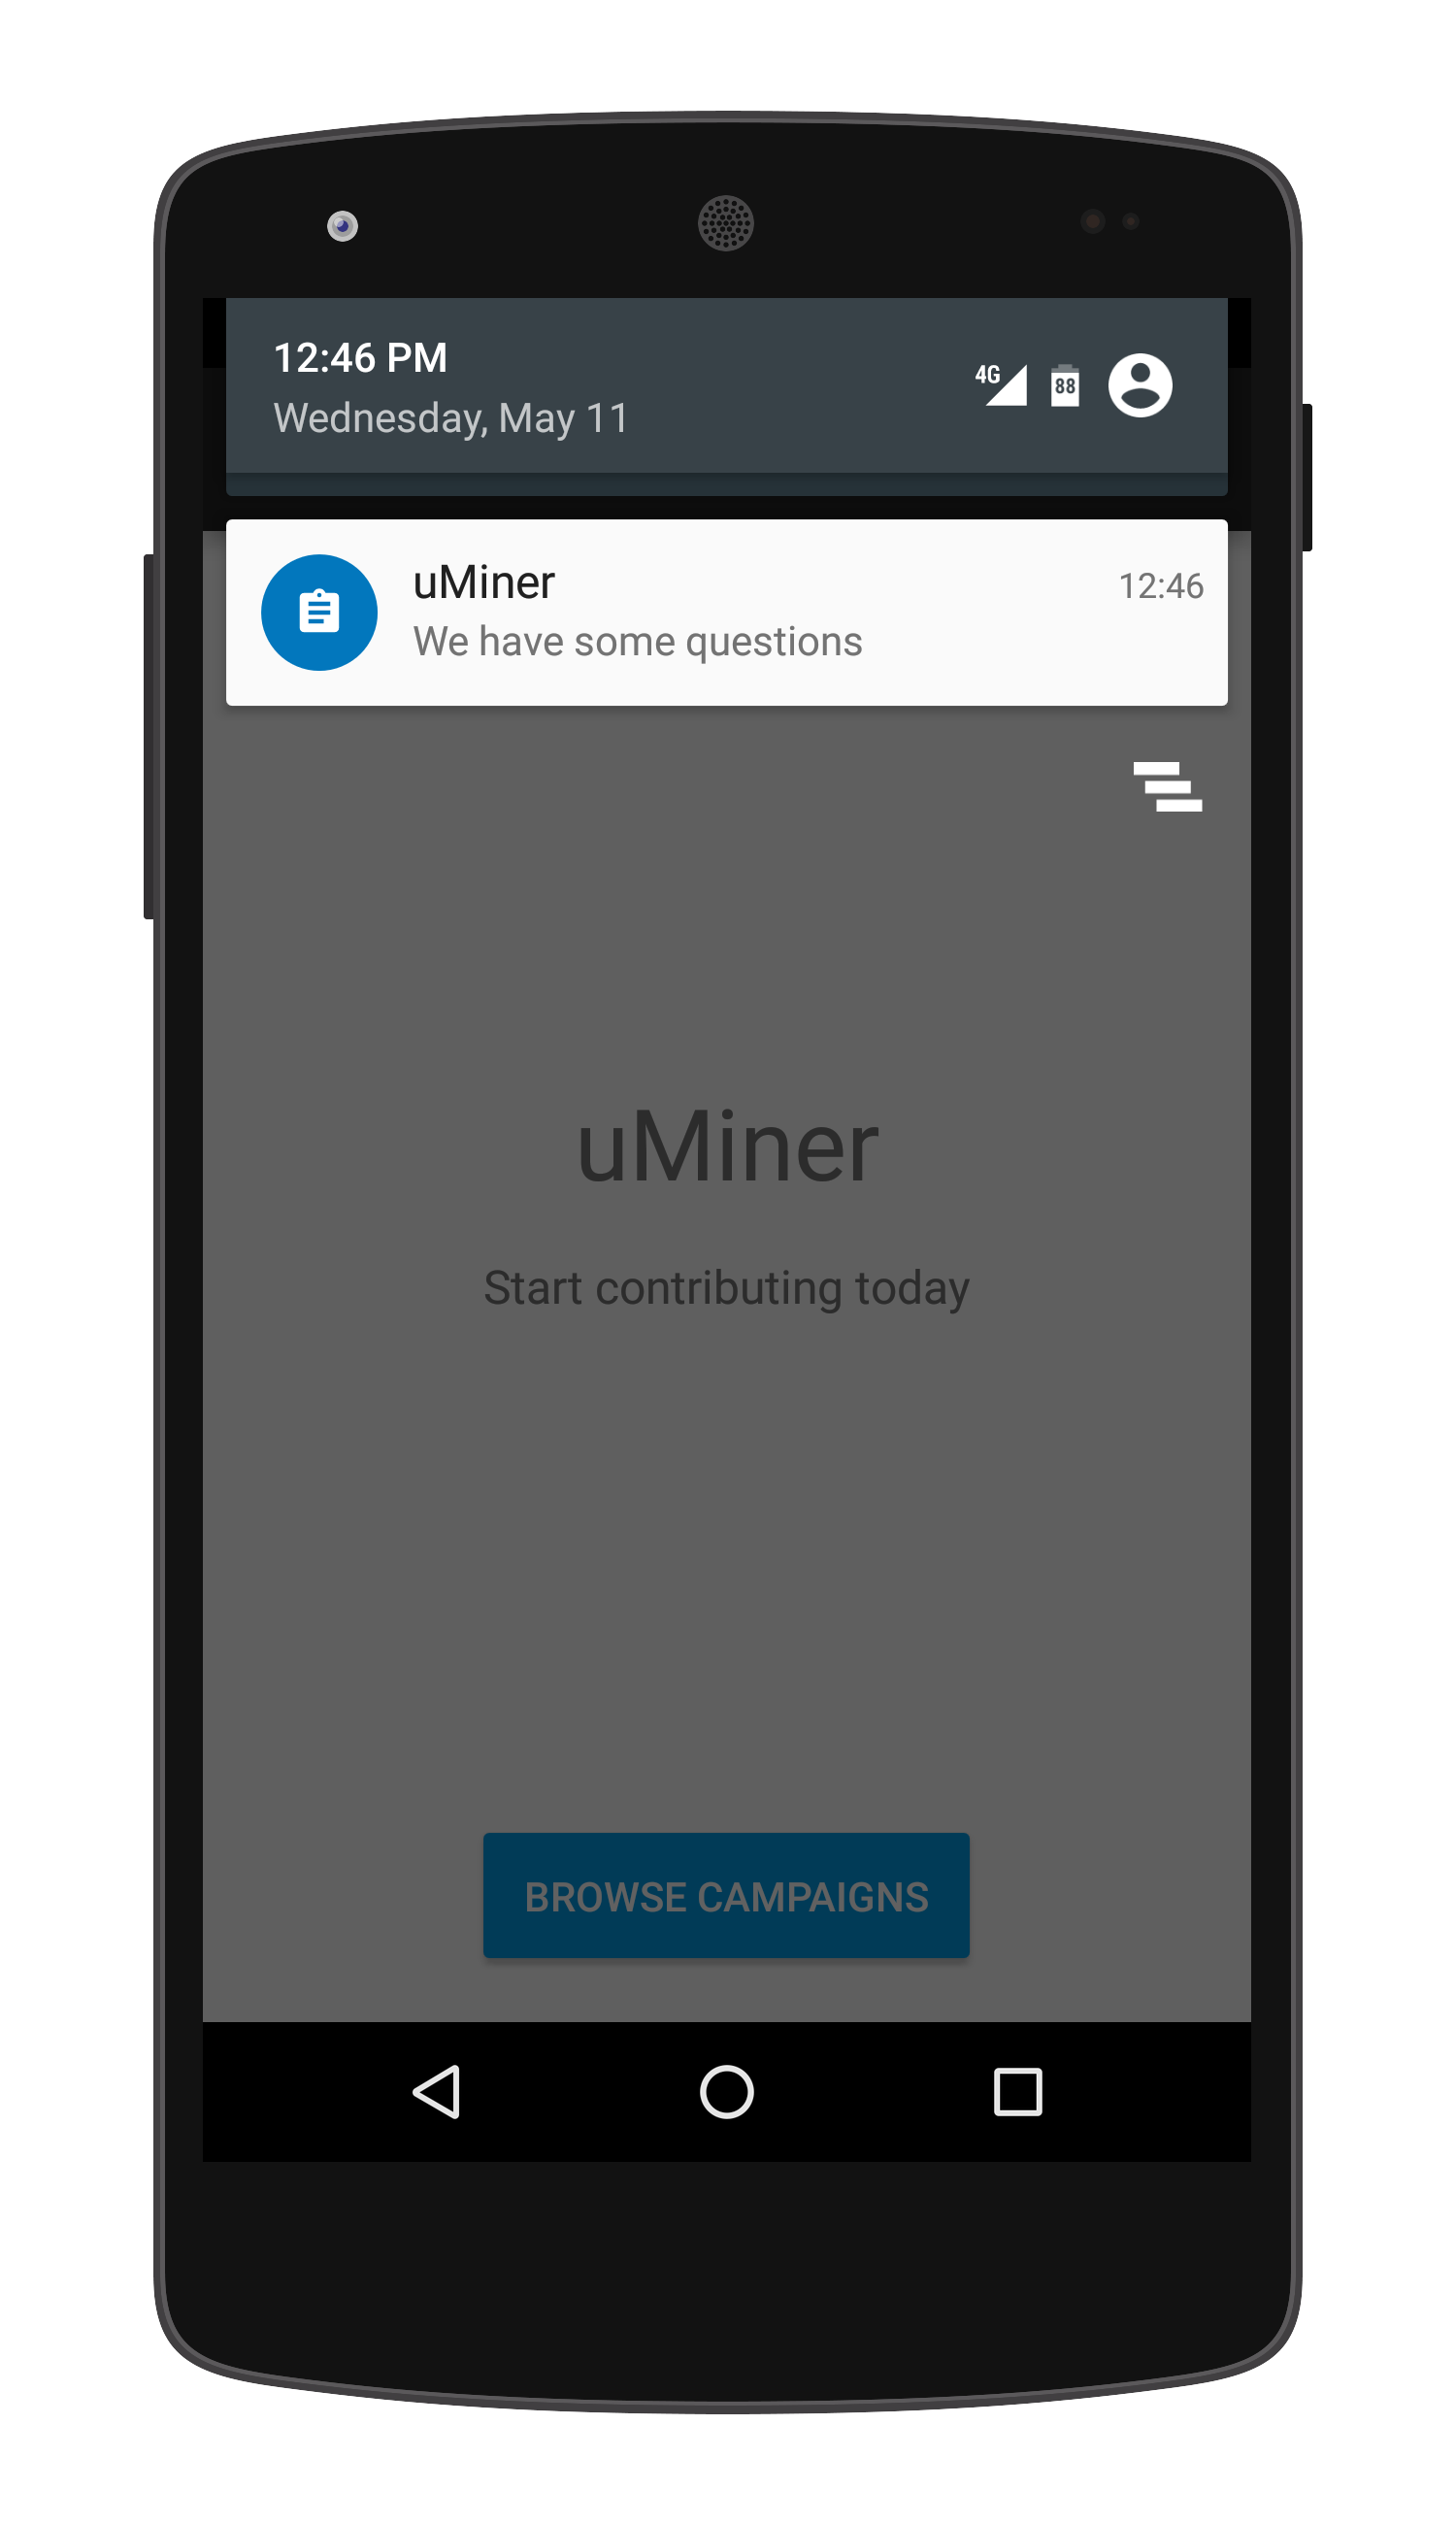
\includegraphics[width=.73\linewidth]{user_interfaces/client/client_notification_with_phone}
        \caption{Notification to answer questions.}
        \label{fig:answering_questionnaire_notification}
    \end{subfigure}%
    \begin{subfigure}[!t]{.50\textwidth}
        \centering
        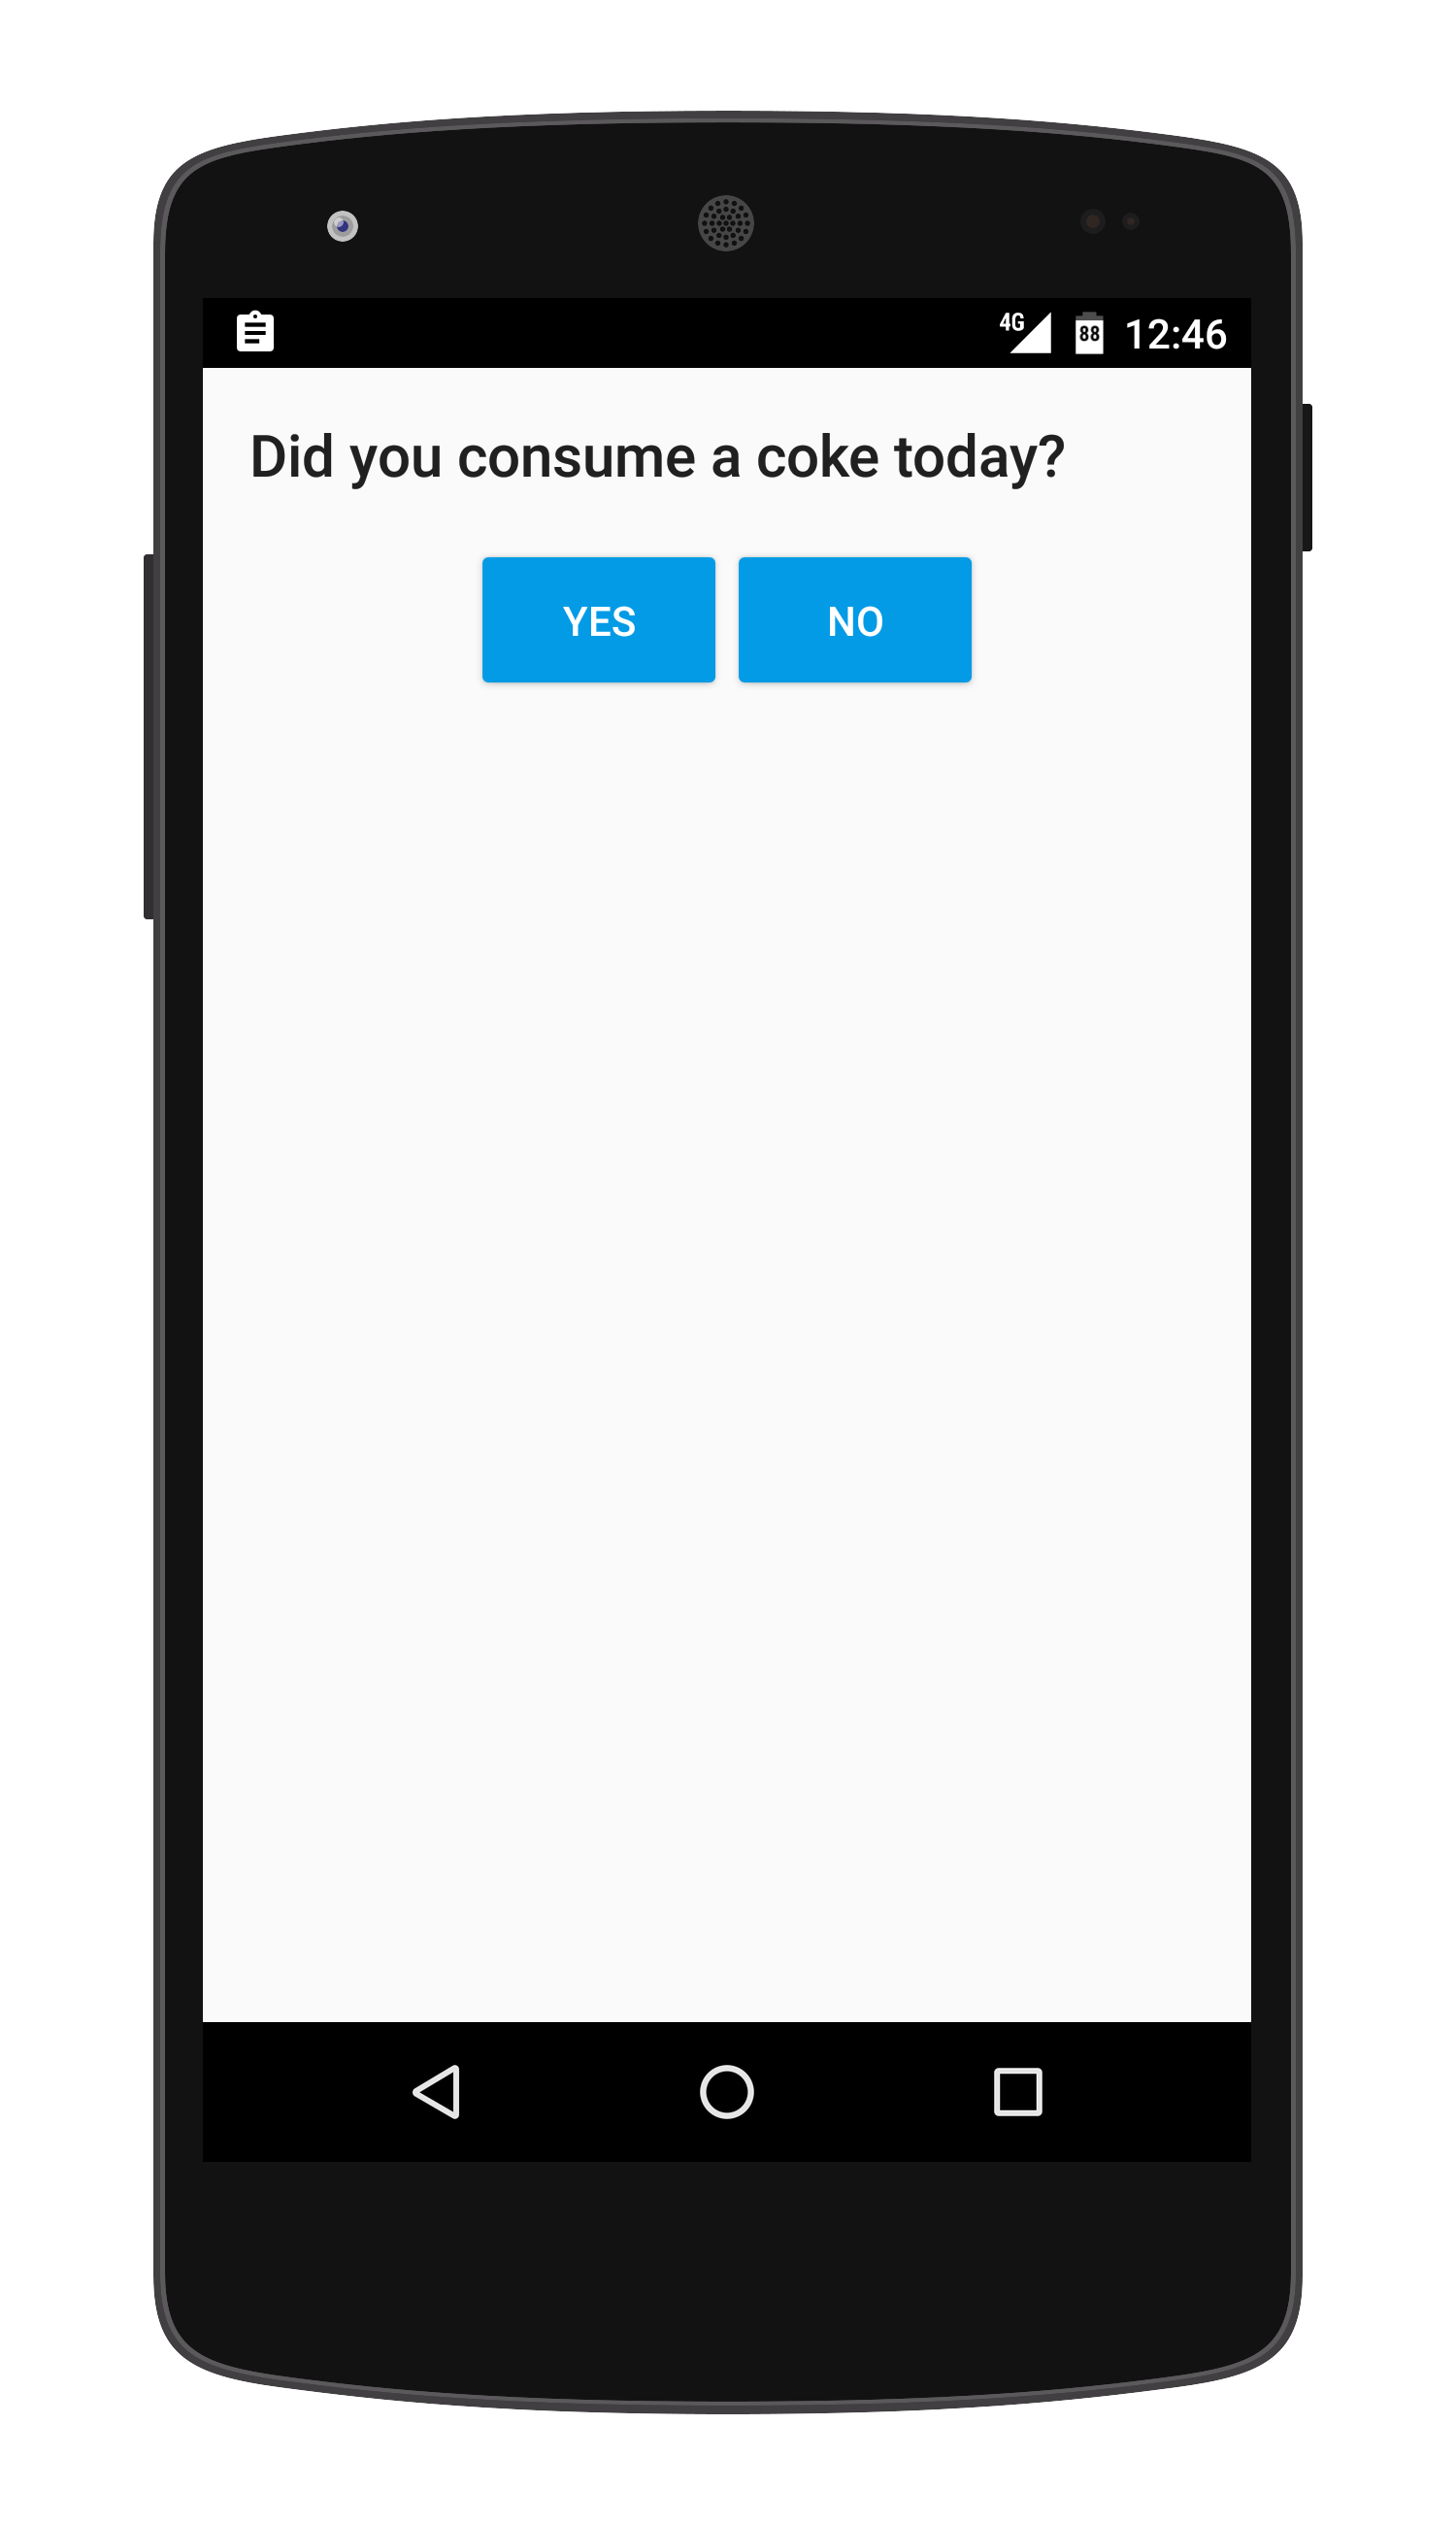
\includegraphics[width=.73\linewidth]{user_interfaces/client/client_answering_questions_with_phone}
        \caption{View when answering a question.}
        \label{fig:answering_questionnaire_answering}
    \end{subfigure}
    \caption{Questionnaire notification which is ready to be answered and view of a question being answered.}
    \label{fig:answering_questionnaire}
\end{figure}
\FloatBarrier

In the current implementation of the system, customers can only specify yes/no questions, but we have thought of different concepts for getting labels for snapshots:

\begin{description}
    \item[Complex questions] might be required for customers to get a better understanding of the label. Such questions could be: \emph{Which of the following statements would describe your current situation best?} or \emph{Please provide a small description of your current mood}. Questions such as the latter might be harder for customers to interpret automatically, but techniques such as sentiment analysis \parencite{pang2008opinion} could be applied here. The system should, ideally, not limit the customer in defining what label they would like to retrieve, i.e. customers should be able to define their own kind of question, or activity, they wish for participants to perform. 

    \item[Answer dependent questions] might be desired by customers to get a more detailed label, e.g. if the participants answers \emph{yes} to $q_1$, ask him $q_2$, otherwise ask $q_3$. Defining questions depending on the outcome of previous questions could become a complex task, and the customers might need visual aid in the creation of such questions.
    \\\\
    The customer interface might utilize some kind of drag and drop programming, like the programming platform for Lego Mindstorm\footnote{http://www.lego.com/da-dk/mindstorms/learn-to-program} to design questionnaires. With this the customer would be able to design the questionnaire just the way they want it, and be able to define exactly how they want to have their snapshots labeled. 
\end{description}
\newpage
In the current application, questionnaires are triggered, and showed to the user, either in the start or the end of a snapshot, as described in \secref{sec:temporal_properties_of_snapshots}. This will cause the time of questionnaires to be relative to the time that the participants subscribed to the campaign. Some customers might instead be interested in questionnaires occurring at certain points of the day or occur when some event occur. Therefore we have considered some alternatives for triggering the questionnaires.

\begin{description}
    \item[Timely fixed triggers] might be useful to ensure that all participants are notified regarding questionnaires simultaneously, i.e. at a specific time of day. This might cause gathered information to be more easily related. Furthermore, customers might be interested in asking participants regarding something, only at a specific time, e.g. at eight in the morning. 

    \item[Event triggers] could be useful since participants is answering questions based on their own memory. So instead of waiting a fixed amount of time, triggers could be event based. This would prompt participants to answer questionnaires when a specific event occurs, e.g. when returning home, after finishing a call, or when a sensor reads a major fluctuation etc.    
\end{description}    

%!TEX root = ../../super_main.tex

\section{Customer Interaction}
\label{sec:customer_interaction}
To provide customers with a way of defining campaigns, and retrieving information from the system, a website has been created. This website is only available to customers, who may interact with the system in two ways, depending on their intent. Customers can, through a GUI, browse their campaigns as well as create new ones. Alternatively, if customers wish to retrieve the snapshots for a campaign, they may retrieve it in a JSON format. Both ways of interacting with the system will be described in this section. Mockups of the customer GUI can be found in \appref{app:web_mockup}.   
\\\\
The interface for the customer is meant to be an expert system, where more explicit training in how to use the system might be necessary. This has been decided as we deem that the customers in need of snapshots will be willing to invest more effort into using the system in order to get the snapshots they desire. This means that some part of the system might be less intuitive and will require some kind of tacit knowledge to be productive when using it. 
\\\\
Note that screenshots of the UI, where the address bar of the browser window is visible, show the base URL \mono{https://prod.local.element67.dk:8000}. This URL can be used to visit the website on the university network. However, if you want to visit the site from outside the network you will need to use another URL, namely \mono{https://prod.global.element67.dk:8000}. 
\\\\
When visiting the site, customers are presented with the page seen in \figref{fig:web_welcome}. Everybody, meaning both customers, participants, and people outside these categories, have access to this page. This means that it could be utilized to give the visitors more information regarding the system and be used as a promotion site for the uMiner platform. 

% Welcome not logged in
\begin{figure}[!htbp]
\centering
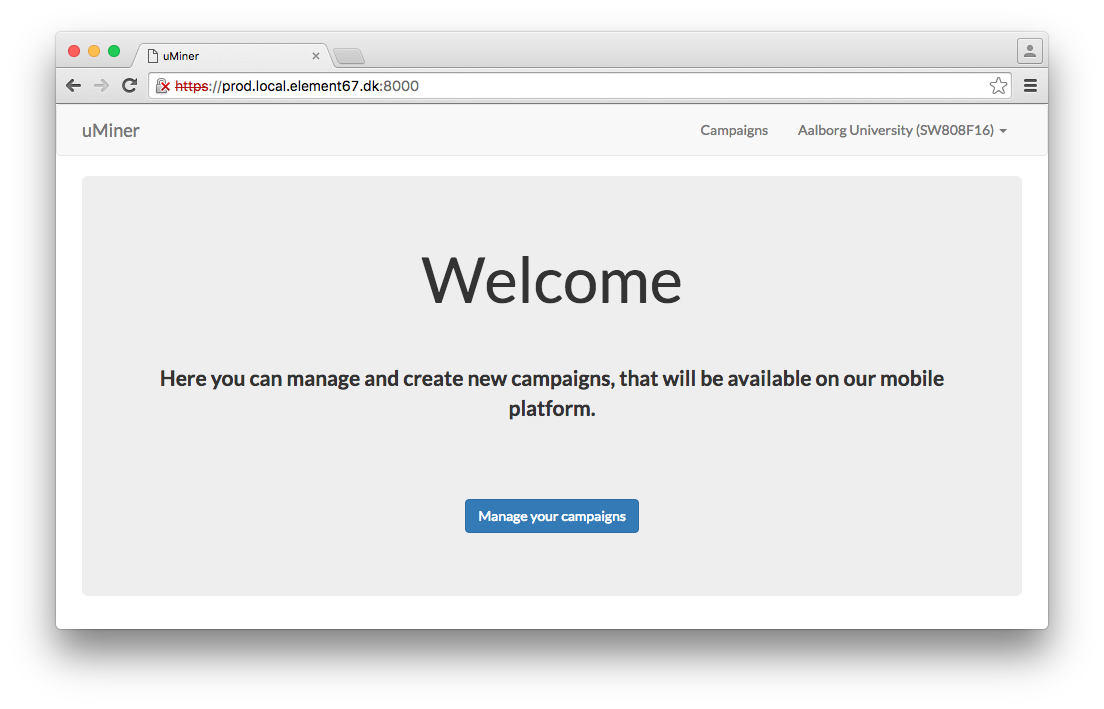
\includegraphics[width=\linewidth]{user_interfaces/web/web_welcome}
\caption{Welcome page.}
\label{fig:web_welcome}
\end{figure}
\FloatBarrier

\subsection{Registration and Logging In}

To gain access to the features of the website, customers must firstly log in. If the customer does not have a login, he can create one. The page for registration as well as the login page are similar to the ones of many other pages. When a user registers he is asked to provide a name, an email and a password. The name is used to show participants who created the different campaigns, allowing them to pick and choose which customers they wish to contribute data to. Please note that the same name can be shared by multiple accounts. This means that multiple accounts can be associated with \emph{Aalborg University}, for instance. Currently, everybody can register an account, but one could imagine that some level of verification might be required, so people cannot impersonate companies or persona. Furthermore, one could imagine that multiple users would like to have access to the same customer-login without having to share the same password. Because of this, it might be beneficial to implement a feature, where multiple accounts would have access to the same campaigns and snapshots.

% % Register
% \begin{figure}[!htbp]
% \centering
% 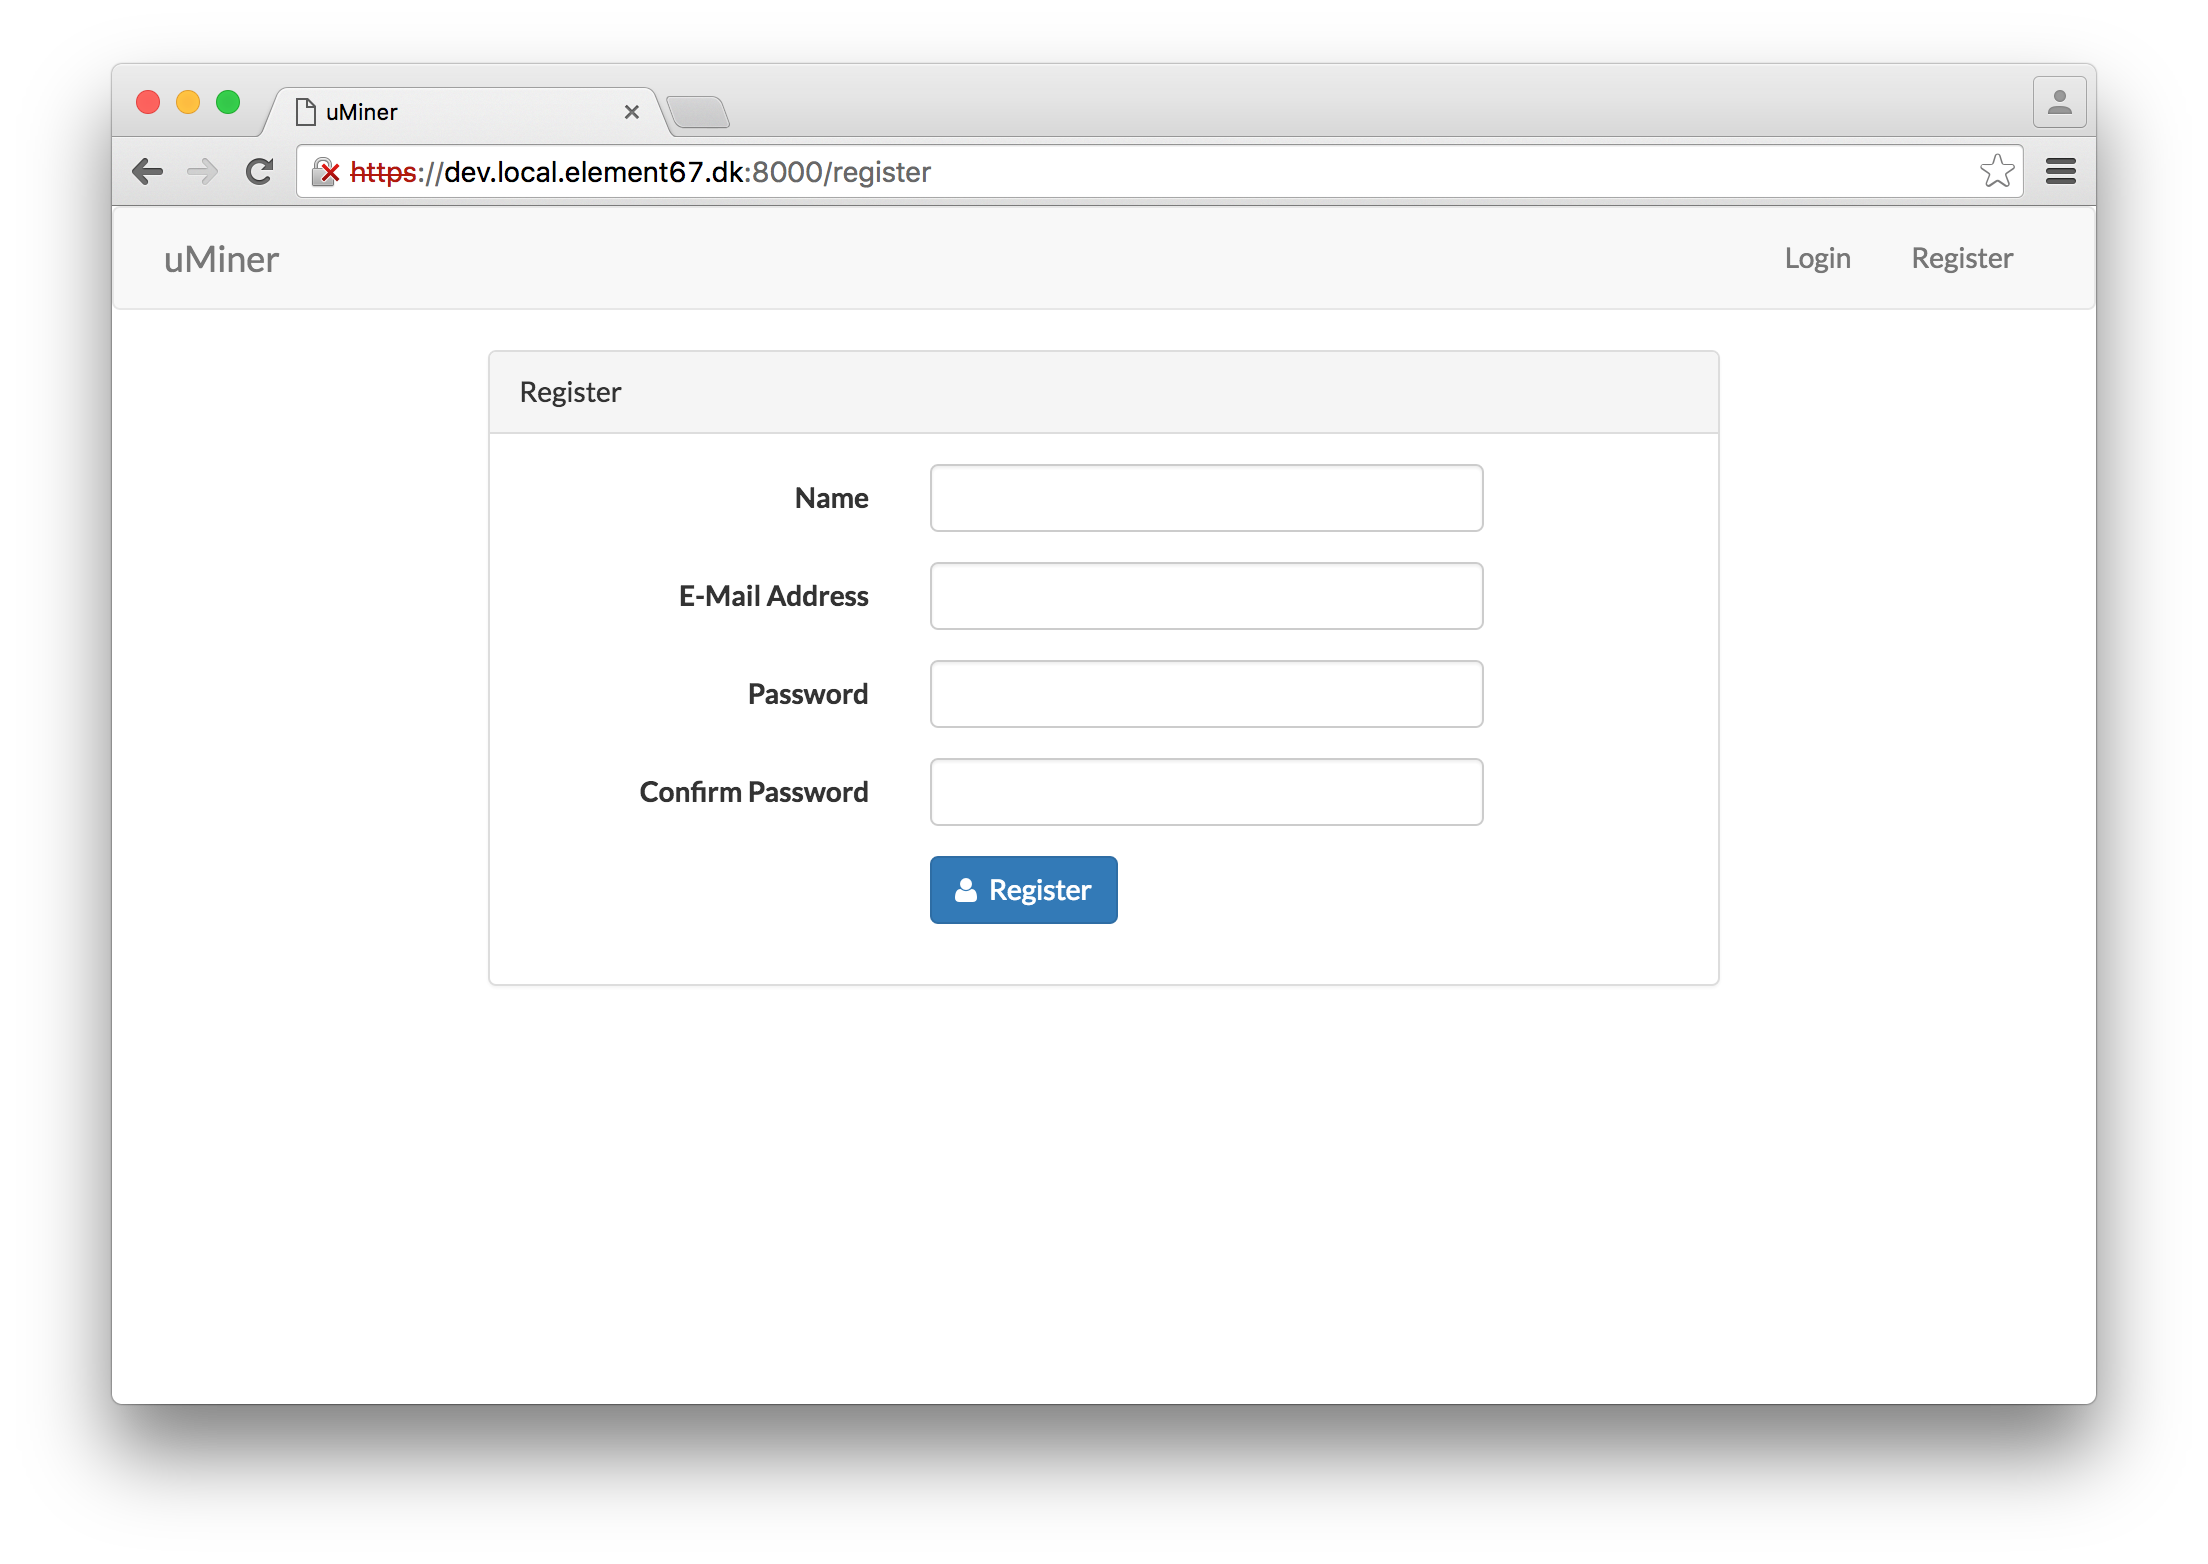
\includegraphics[width=\linewidth]{user_interfaces/web/web_register}
% \caption{Register page.}
% \label{fig:web_register}
% \end{figure}
% \FloatBarrier

% % Login
% \begin{figure}[!htbp]
% \centering
% 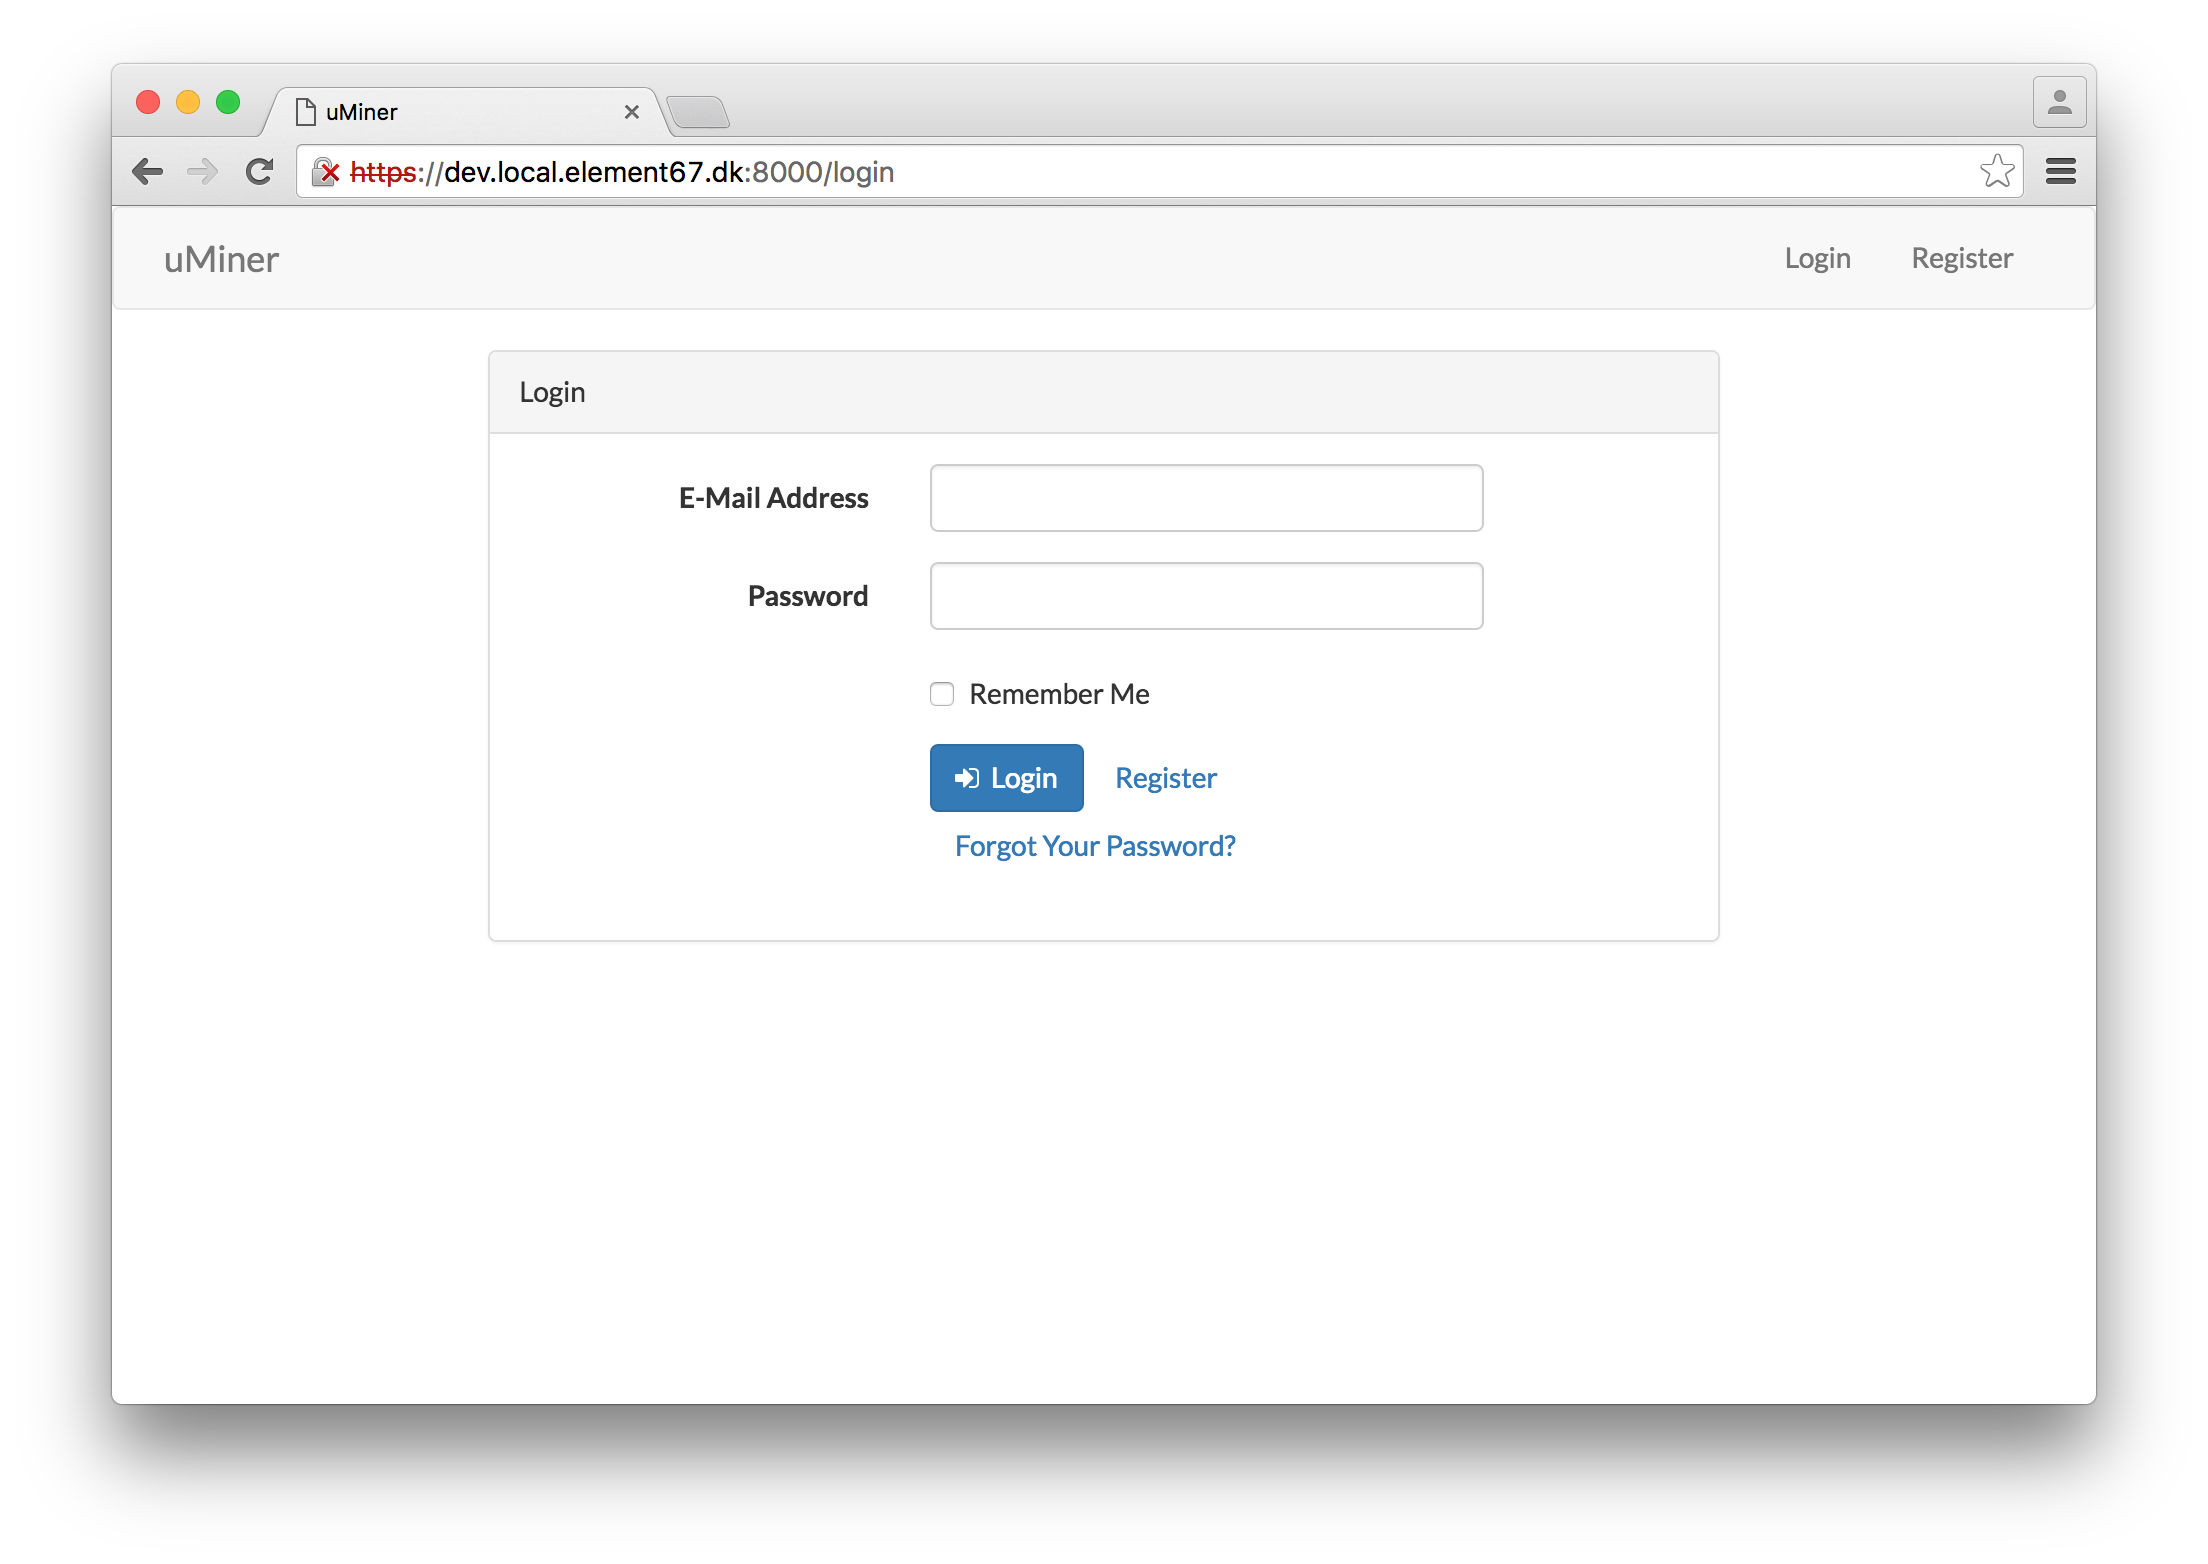
\includegraphics[width=\linewidth]{user_interfaces/web/web_login}
% \caption{Login page.}
% \label{fig:web_login}
% \end{figure}
% \FloatBarrier

\subsection{Creating Campaigns}
\label{sub:creating_campaign}

When a customer is logged in, he has the option to create campaigns. This is done through the site seen in \figref{fig:web_create_campaign}. Here, customers will have to specify different details regarding the campaign. To give customers an idea of how the participants will view this information, an example of campaign viewed in the Android application is included on the page. In order for customers to create a campaign, the following information can be provided:

\begin{description}
    \item[Campaign title] is used to give participants a rough idea of what the campaign will be used for. This information will visible when participants are browsing campaigns and when viewing details regarding a campaign.

    \item[Campaign description] will provide participants with a detailed description of the campaign and its purpose. This text could possibly also contain motivational factors, inclining participants to contribute to the given campaign. This information is only available to participants when viewing the specifications of the campaign.

    \item[Campaign author] cannot be specified directly by the customer, but is instead depending on the name of the customer as specified in his account credentials. Like the campaign title, this information will be included when participants are browsing campaigns, and when viewing details regarding the campaign.

    \item[Campaign availability] can be specified through the checkbox directly below the description input field. This checkbox is marked by default, making the campaign publicly available, meaning that it is visible for participants when they are browsing the campaigns (see \figref{fig:public_campaigns}). Unchecking this checkbox will cause the campaign to be private, 
    meaning that it will not be visible in the list of public campaigns on the participant's device, effectively meaning that customers will have to distribute the campaign identifier in order to get participants.

    \item[Sensors] allows the customer to specify, which sensors they would like to gather information from. Sensors are divided into four categories, which roughly describes the information that the sensors will collect. In the current implementation participants can join any campaign even though their phone does not have all of the sensors the customer has specified. Customers might be interested in excluding participants, who does not have some essential sensors.

    \item[Sample and measurement] consists of five different input fields. The \emph{Snapshots per Campaign} input is used to specify how many snapshots the participant must collect before completing a campaign.

    The \emph{Measurement per Sample}- and \emph{Measurement delay} input fields will change the length of a sample, while the \emph{Samples per Snapshot}- and \emph{Sample delay} input fields will change the length of a Snapshot. Please note that this way of specifying snapshots differs from the internal structure, explained in \secref{sec:temporal_properties_of_snapshots}. We did this, since we deemed it easier to specify the delay between measurements and samples, rather than having to calculate the different frequencies.

    The concept of delay, amount of measurements, samples etc. might still be difficult to grasp, so we have included a illustration of a time line. This could possibly aid customers in specifying the different parameters, and represent how a snapshot is structured (see \figrefpage{fig:sample_temporality}). Ideally, the figure should be responsive by automatically updating whenever customers change the provided information.

    \item[Questionnaire placement] will indicate when participants are prompted with questions. As described previously, in \secref{sub:answering_questionnaired}, this can either be in the beginning, or at the end of a snapshot. 

    \item[Questionnaire] consists of a sequence of questions. Questions can be re-arranged by dragging them up or down in the list. The participants will receive the questions in the order they are presented on this page. If a customer does not specify any question to his/her campaign, the participants will never be prompted to fill out a questionnaire if they have joined that campaign.
\end{description}

% Create campaign
\begin{figure}[!htbp]
\centering
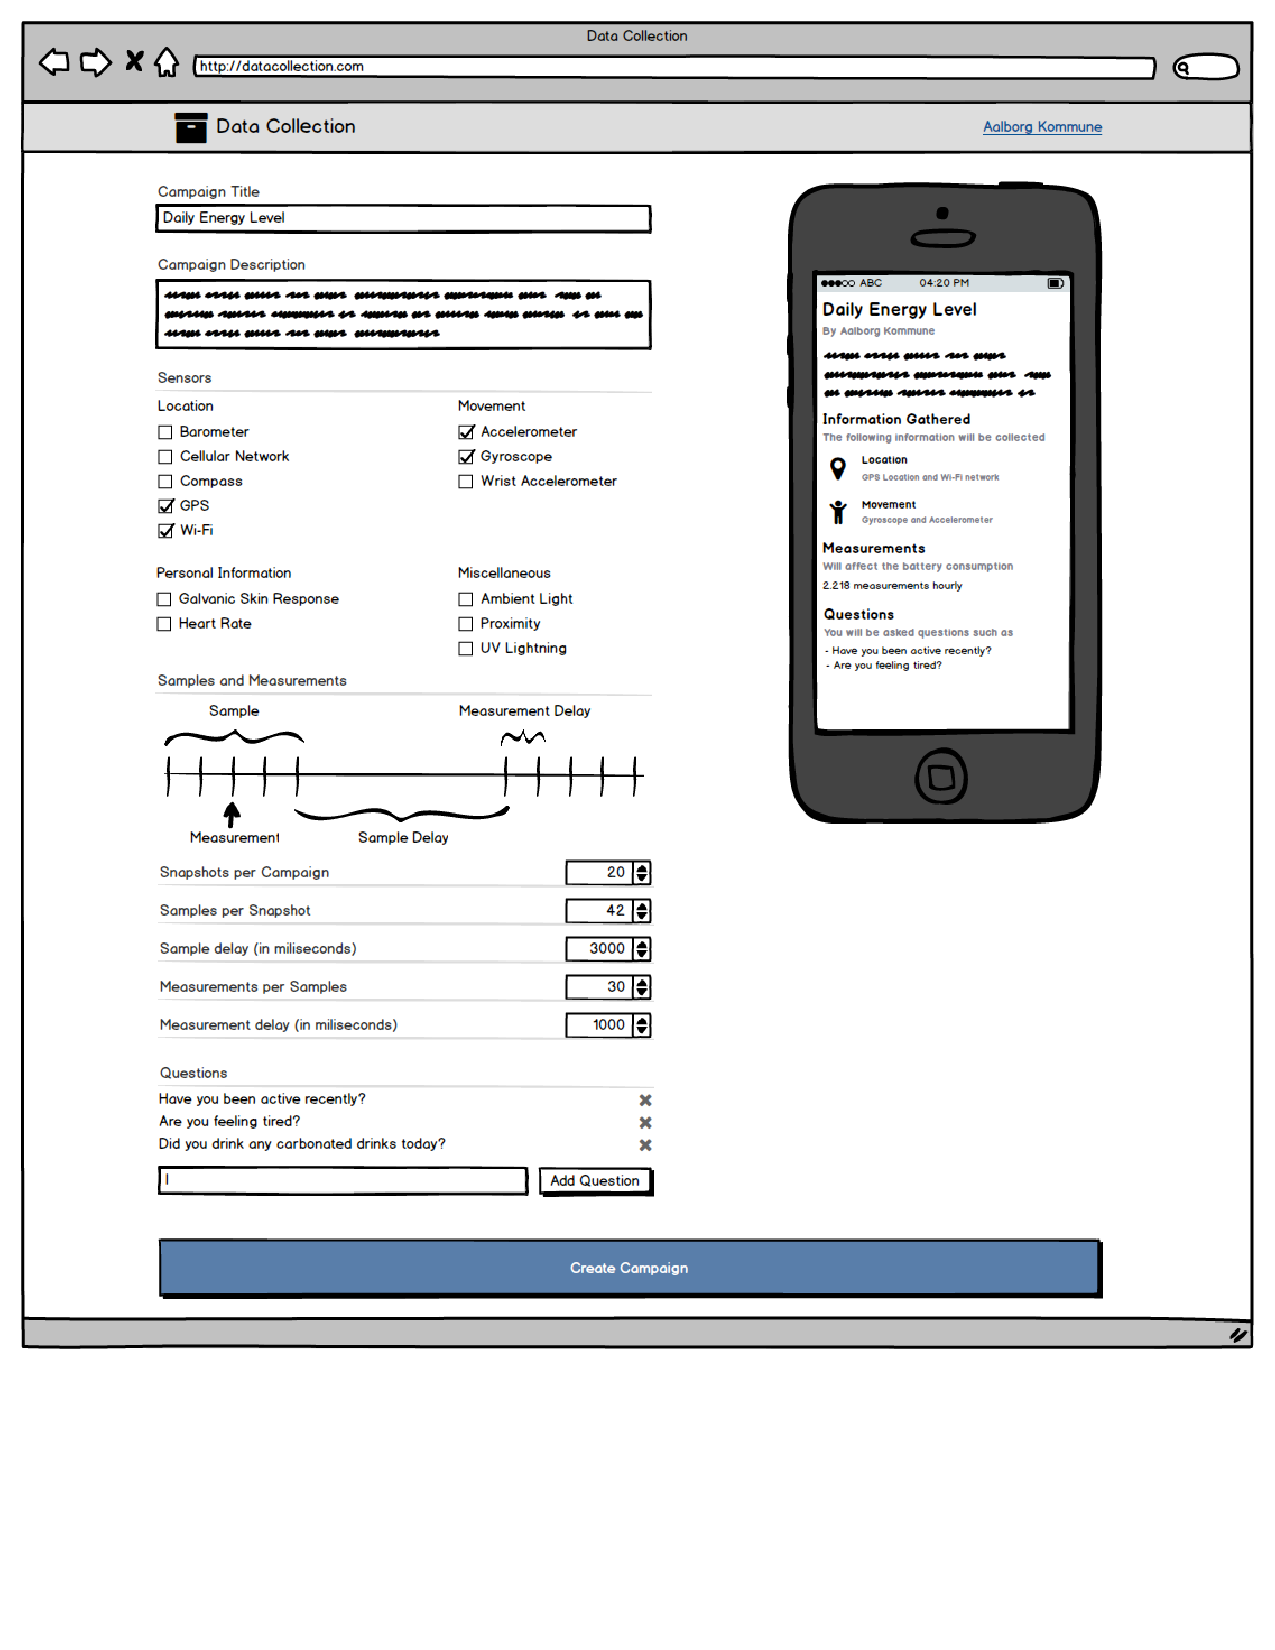
\includegraphics[width=\linewidth]{user_interfaces/web/web_create_campaign}
\caption{The creation of the campaign \emph{Alcohol and You}.}
\label{fig:web_create_campaign}
\end{figure}
\FloatBarrier

\subsection{Viewing Campaign Details and Gathered Snapshots}
\label{sub:viewing_campaign_details}

When customers have created a campaign, it will show up in their list of campaigns, as seen in \figref{fig:web_view_campaigns}. If the customer have not created any campaigns yet, this page will only contain the small description along with the \emph{Create}-button. If the customer presses any of the created campaigns on this page, he will be redirected to a page similar to the one seen in \figref{fig:web_view_campaign}. This page will reflect the values the customer inputted when he created the campaign through the creation page. Furthermore, the page also contains the identifier of the campaign, that the customer can distribute, through other media than our application, to potential participants. On the right side of the page, a \emph{Progress} area has been included. We have included this so customers may get an insight in on how many participants have contributed (\emph{Participants joined}), but also much data has been collected and uploaded to the server (\emph{Snapshots submitted}). One could imagine that it would be possible to extend the system with additional useful metrics, for example displaying the most common time that participants answer questions, which questions makes them close the application, etc. 

% View campaigns
\begin{figure}[!htbp]
\centering
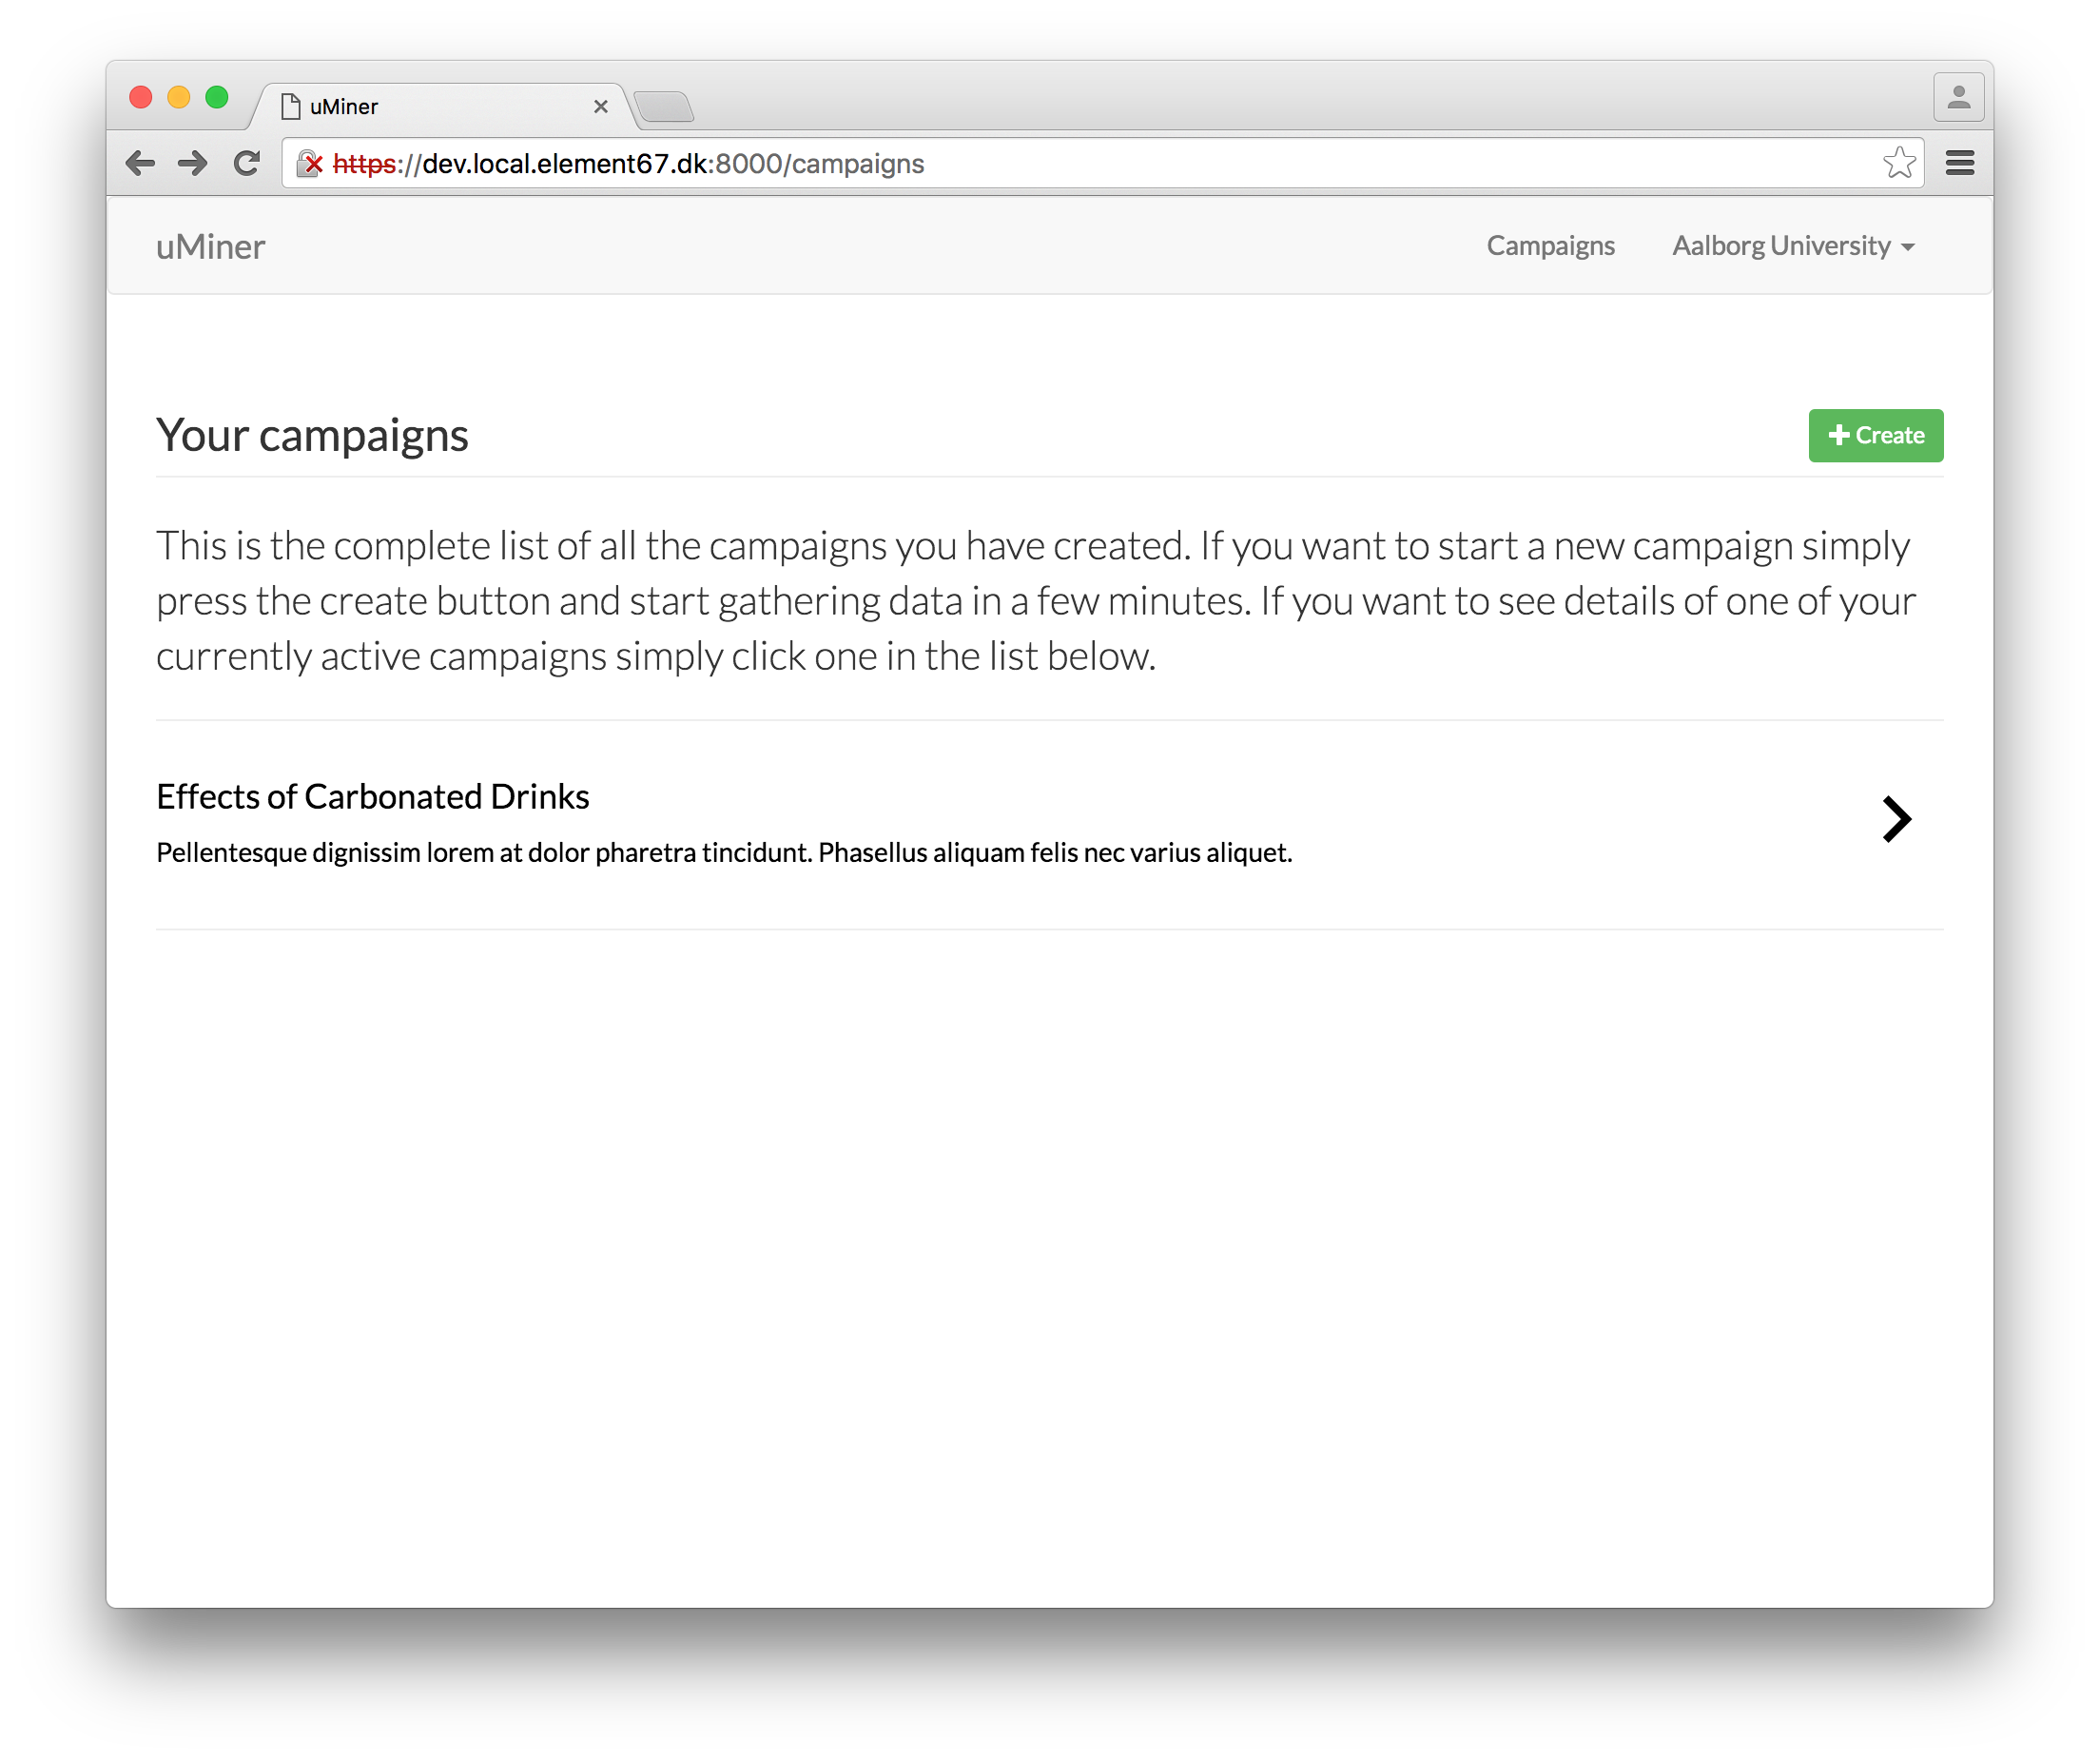
\includegraphics[width=\linewidth]{user_interfaces/web/web_view_campaigns}
\caption{The list of campaigns for the \emph{Aalborg University} user.}
\label{fig:web_view_campaigns}
\end{figure}
\FloatBarrier

% View specific campaign
\begin{figure}[!htbp]
\centering
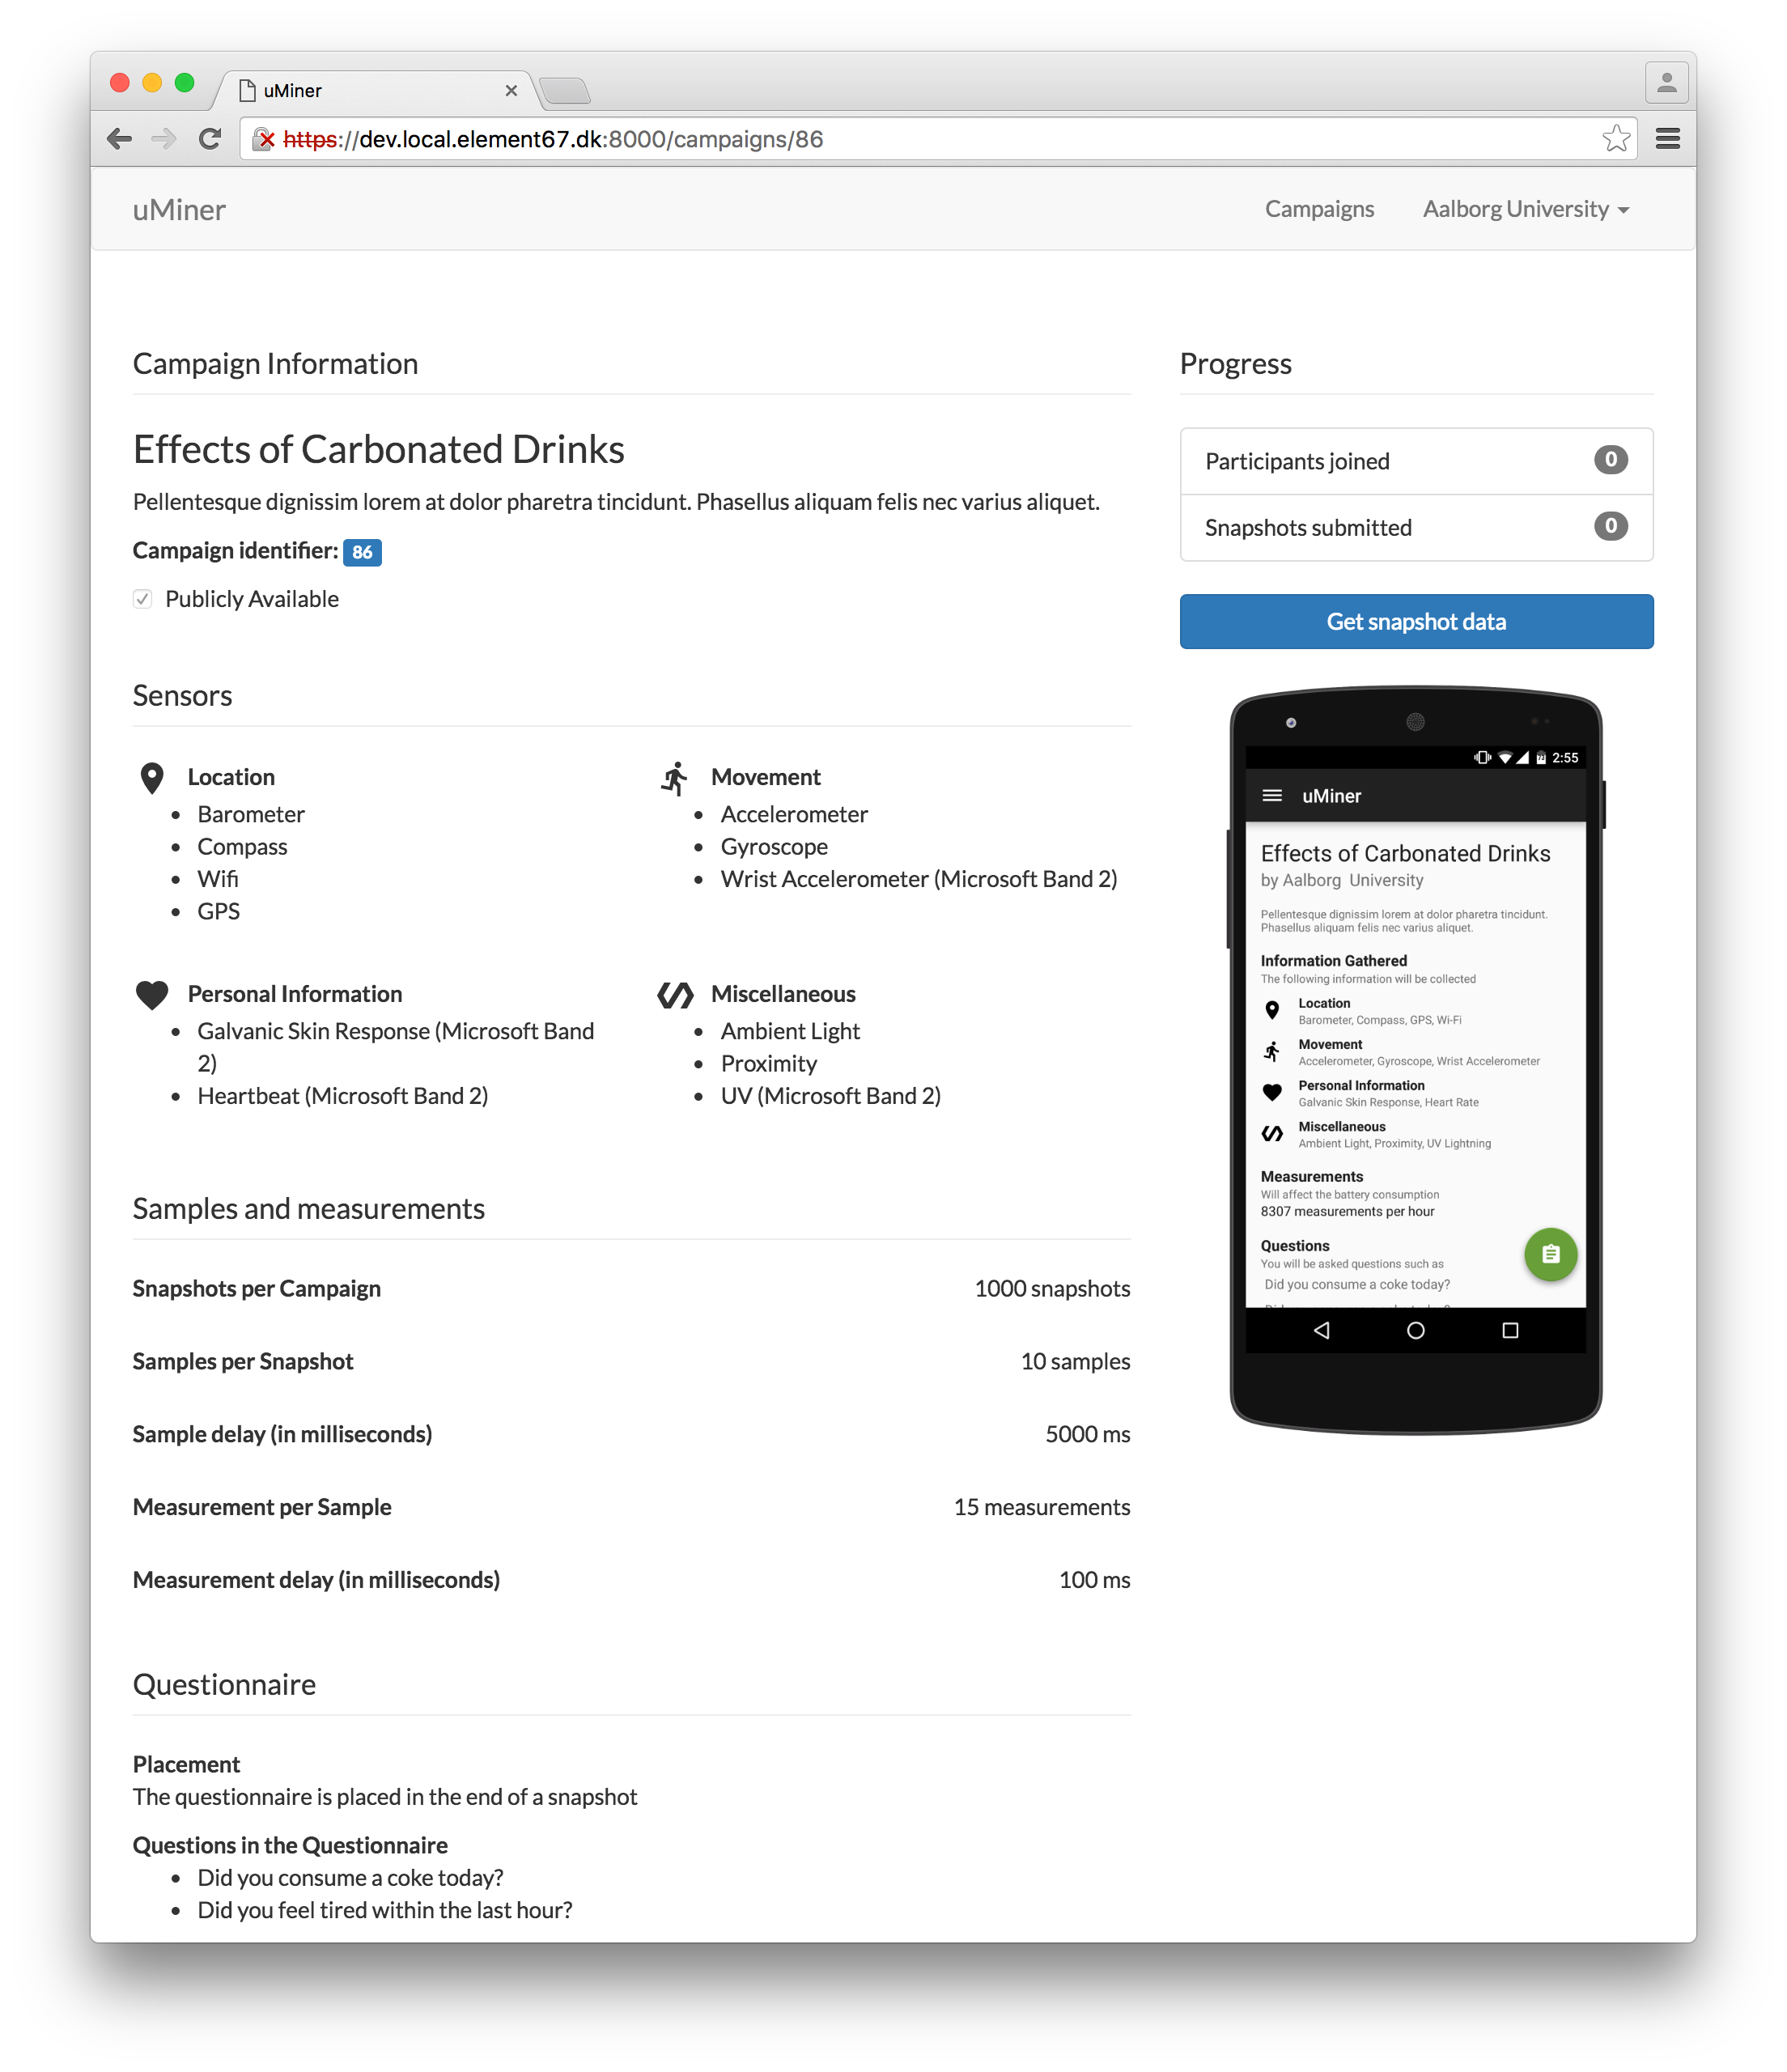
\includegraphics[width=\linewidth]{user_interfaces/web/web_view_campaign}
\caption{Viewing details regarding specific campaign.}
\label{fig:web_view_campaign}
\end{figure}
\FloatBarrier

To view the collected snapshots, submitted by the application, customers can press the \emph{Get snapshot data} button, just below the statistics. This will redirect the user to a site, containing unformatted JSON, describing the different snapshots that have been contributed to that particular campaign. \lstref{lst:snapshot_json_example} shows the structure of the JSON output. The first few entries in the object will describe some meta-information about the snapshots collected, such as the total amount of snapshots collected (\mono{total}). Furthermore, these objects will also describe how to iterate through the data set through pagination, for instance the \mono{per\_page} entry will specify how many snapshots will be displayed per page. To retrieve the next set of snapshots, the customer will have to visit the page specified in the \mono{next\_page\_url} entry. The collected snapshots are stored in the array with the key \mono{data}. An entry in this array contains a snapshot object (\mono{snapshot}), but also consists of some meta-information, such as who submitted it (\mono{participant\_id}), when it was submitted (\mono{created\_at}) etc. 

\lstinputlisting[
   style = json,
   caption = {Illustration of the JSON structure of collected snapshots.},
   label = {lst:snapshot_json_example},
   float=!htbp,
]{content/user_interface/code_snippets/snapshot_json_example.json}
\FloatBarrier

\subsection{Deleting and Editing Campaigns}
\label{sub:editing_and_deleting_campaigns}
In order to delete a campaign, customers will have to press the red \emph{Delete} button, which can be seen in \figref{fig:web_view_campaign}. In the current implementation of the system, it is not possible to edit campaigns, since we deemed it to be an less wanted feature for the project. This decision was based on the fact that there would be no difference in editing the campaign and deleting and recreating the campaign. A problem with the edit functionality is, if a customer choose to edit a campaign, all the participants who are subscribed to that campaign would have to be notified that the campaign has being edited, and they might not be able to accept the edited campaign, and would have to be forced to unsubscribe from it. Furthermore, all the gathered snapshots might have to be invalidated, need to be removed, or otherwise marked as belonging to an older version, because there might be missing sensors or labels. It is possible to implement checks, that would inform the participants regarding the updated campaign, asking them to re-subscribe to the campaign. 
\\\\
It is easy to imagine that customers would like to update the title, description, or the questions to correct spelling errors, or give a better clarification of the campaign. This would not require the removal of already collected data, since it would not be invalidated, because the semantics of the labels would not change. However, we choose not to pursue any of these editing solutions, and instead focus on the underlying system to obtain a minimum viable product. 